% Options for packages loaded elsewhere
\PassOptionsToPackage{unicode}{hyperref}
\PassOptionsToPackage{hyphens}{url}
%
\documentclass[
]{book}
\usepackage{amsmath,amssymb}
\usepackage{iftex}
\ifPDFTeX
  \usepackage[T1]{fontenc}
  \usepackage[utf8]{inputenc}
  \usepackage{textcomp} % provide euro and other symbols
\else % if luatex or xetex
  \usepackage{unicode-math} % this also loads fontspec
  \defaultfontfeatures{Scale=MatchLowercase}
  \defaultfontfeatures[\rmfamily]{Ligatures=TeX,Scale=1}
\fi
\usepackage{lmodern}
\ifPDFTeX\else
  % xetex/luatex font selection
\fi
% Use upquote if available, for straight quotes in verbatim environments
\IfFileExists{upquote.sty}{\usepackage{upquote}}{}
\IfFileExists{microtype.sty}{% use microtype if available
  \usepackage[]{microtype}
  \UseMicrotypeSet[protrusion]{basicmath} % disable protrusion for tt fonts
}{}
\makeatletter
\@ifundefined{KOMAClassName}{% if non-KOMA class
  \IfFileExists{parskip.sty}{%
    \usepackage{parskip}
  }{% else
    \setlength{\parindent}{0pt}
    \setlength{\parskip}{6pt plus 2pt minus 1pt}}
}{% if KOMA class
  \KOMAoptions{parskip=half}}
\makeatother
\usepackage{xcolor}
\usepackage{color}
\usepackage{fancyvrb}
\newcommand{\VerbBar}{|}
\newcommand{\VERB}{\Verb[commandchars=\\\{\}]}
\DefineVerbatimEnvironment{Highlighting}{Verbatim}{commandchars=\\\{\}}
% Add ',fontsize=\small' for more characters per line
\usepackage{framed}
\definecolor{shadecolor}{RGB}{248,248,248}
\newenvironment{Shaded}{\begin{snugshade}}{\end{snugshade}}
\newcommand{\AlertTok}[1]{\textcolor[rgb]{0.94,0.16,0.16}{#1}}
\newcommand{\AnnotationTok}[1]{\textcolor[rgb]{0.56,0.35,0.01}{\textbf{\textit{#1}}}}
\newcommand{\AttributeTok}[1]{\textcolor[rgb]{0.13,0.29,0.53}{#1}}
\newcommand{\BaseNTok}[1]{\textcolor[rgb]{0.00,0.00,0.81}{#1}}
\newcommand{\BuiltInTok}[1]{#1}
\newcommand{\CharTok}[1]{\textcolor[rgb]{0.31,0.60,0.02}{#1}}
\newcommand{\CommentTok}[1]{\textcolor[rgb]{0.56,0.35,0.01}{\textit{#1}}}
\newcommand{\CommentVarTok}[1]{\textcolor[rgb]{0.56,0.35,0.01}{\textbf{\textit{#1}}}}
\newcommand{\ConstantTok}[1]{\textcolor[rgb]{0.56,0.35,0.01}{#1}}
\newcommand{\ControlFlowTok}[1]{\textcolor[rgb]{0.13,0.29,0.53}{\textbf{#1}}}
\newcommand{\DataTypeTok}[1]{\textcolor[rgb]{0.13,0.29,0.53}{#1}}
\newcommand{\DecValTok}[1]{\textcolor[rgb]{0.00,0.00,0.81}{#1}}
\newcommand{\DocumentationTok}[1]{\textcolor[rgb]{0.56,0.35,0.01}{\textbf{\textit{#1}}}}
\newcommand{\ErrorTok}[1]{\textcolor[rgb]{0.64,0.00,0.00}{\textbf{#1}}}
\newcommand{\ExtensionTok}[1]{#1}
\newcommand{\FloatTok}[1]{\textcolor[rgb]{0.00,0.00,0.81}{#1}}
\newcommand{\FunctionTok}[1]{\textcolor[rgb]{0.13,0.29,0.53}{\textbf{#1}}}
\newcommand{\ImportTok}[1]{#1}
\newcommand{\InformationTok}[1]{\textcolor[rgb]{0.56,0.35,0.01}{\textbf{\textit{#1}}}}
\newcommand{\KeywordTok}[1]{\textcolor[rgb]{0.13,0.29,0.53}{\textbf{#1}}}
\newcommand{\NormalTok}[1]{#1}
\newcommand{\OperatorTok}[1]{\textcolor[rgb]{0.81,0.36,0.00}{\textbf{#1}}}
\newcommand{\OtherTok}[1]{\textcolor[rgb]{0.56,0.35,0.01}{#1}}
\newcommand{\PreprocessorTok}[1]{\textcolor[rgb]{0.56,0.35,0.01}{\textit{#1}}}
\newcommand{\RegionMarkerTok}[1]{#1}
\newcommand{\SpecialCharTok}[1]{\textcolor[rgb]{0.81,0.36,0.00}{\textbf{#1}}}
\newcommand{\SpecialStringTok}[1]{\textcolor[rgb]{0.31,0.60,0.02}{#1}}
\newcommand{\StringTok}[1]{\textcolor[rgb]{0.31,0.60,0.02}{#1}}
\newcommand{\VariableTok}[1]{\textcolor[rgb]{0.00,0.00,0.00}{#1}}
\newcommand{\VerbatimStringTok}[1]{\textcolor[rgb]{0.31,0.60,0.02}{#1}}
\newcommand{\WarningTok}[1]{\textcolor[rgb]{0.56,0.35,0.01}{\textbf{\textit{#1}}}}
\usepackage{longtable,booktabs,array}
\usepackage{calc} % for calculating minipage widths
% Correct order of tables after \paragraph or \subparagraph
\usepackage{etoolbox}
\makeatletter
\patchcmd\longtable{\par}{\if@noskipsec\mbox{}\fi\par}{}{}
\makeatother
% Allow footnotes in longtable head/foot
\IfFileExists{footnotehyper.sty}{\usepackage{footnotehyper}}{\usepackage{footnote}}
\makesavenoteenv{longtable}
\usepackage{graphicx}
\makeatletter
\def\maxwidth{\ifdim\Gin@nat@width>\linewidth\linewidth\else\Gin@nat@width\fi}
\def\maxheight{\ifdim\Gin@nat@height>\textheight\textheight\else\Gin@nat@height\fi}
\makeatother
% Scale images if necessary, so that they will not overflow the page
% margins by default, and it is still possible to overwrite the defaults
% using explicit options in \includegraphics[width, height, ...]{}
\setkeys{Gin}{width=\maxwidth,height=\maxheight,keepaspectratio}
% Set default figure placement to htbp
\makeatletter
\def\fps@figure{htbp}
\makeatother
\setlength{\emergencystretch}{3em} % prevent overfull lines
\providecommand{\tightlist}{%
  \setlength{\itemsep}{0pt}\setlength{\parskip}{0pt}}
\setcounter{secnumdepth}{5}
\usepackage{booktabs}
\ifLuaTeX
  \usepackage{selnolig}  % disable illegal ligatures
\fi
\usepackage[]{natbib}
\bibliographystyle{plainnat}
\usepackage{bookmark}
\IfFileExists{xurl.sty}{\usepackage{xurl}}{} % add URL line breaks if available
\urlstyle{same}
\hypersetup{
  pdftitle={Guide R},
  pdfauthor={Prof.~Audrey Bürki, Samuel Arthers, Mégane Bollenrücher},
  hidelinks,
  pdfcreator={LaTeX via pandoc}}

\title{Guide R}
\author{Prof.~Audrey Bürki, Samuel Arthers, Mégane Bollenrücher}
\date{2025-03-12}

\begin{document}
\maketitle

{
\setcounter{tocdepth}{1}
\tableofcontents
}
Merci de prendre note que ce bookdown est en cours de rédaction.

\chapter{Introduction}\label{introduction}

Ceci est le guide R que nous proposons pour vous accompagner durant le cours de Stat I.

\chapter{Installation et environnement R et Rstudio}\label{installation-et-environnement-r-et-rstudio}

\section{Présentation des logiciels}\label{pruxe9sentation-des-logiciels}

R est un langage de programmation adapté au traitement de données et à l'analyse statistique.

Pour programmer en langage R, il est nécessaire d'installer deux outils essentiels:

\begin{enumerate}
\def\labelenumi{\arabic{enumi}.}
\tightlist
\item
  Le \textbf{logiciel R} permet de traduire du texte sous forme de code R en binaire qui est le langage interne du processeur de l'ordinateur.
\item
  Le \textbf{logiciel RStudio} permet de faciliter l'utilisation du logiciel R en donnant l'accès à une interface utilisateur.
\end{enumerate}

Il est possible de faire une analogie avec une voiture. Le logiciel R est le moteur et RStudio est le tableau de bord. Sans le tableau de bord, il n'est pas possible de controler le moteur.

\section{Installation}\label{installation}

\begin{enumerate}
\def\labelenumi{\arabic{enumi}.}
\tightlist
\item
  Installer R sur le site de R.

  \begin{enumerate}
  \def\labelenumii{\roman{enumii}.}
  \tightlist
  \item
    Choisir et télécharger la version de R selon votre système d'exploitation.

    \begin{itemize}
    \tightlist
    \item
      Pour windows : \url{https://cran.r-project.org/bin/windows/base/}
    \item
      Pour MAC : \url{https://cran.r-project.org/bin/macosx/}
    \item
      Pour Linux : \url{https://cran.r-project.org/index.html}
    \end{itemize}
  \item
    Installer le logiciel R sur votre ordinateur en exécutant le fichier téléchargé.
  \end{enumerate}
\item
  Installer RStudio sur le site suivant: \url{https://posit.co/download/rstudio-desktop/}
\end{enumerate}

Après avoir installé ces deux logiciels, vous aurez accès à deux nouvelles applications. Cependant, nous utiliserons uniquement RStudio pour programmer. Lorsque vous exécuterez votre code écrit sur RStudio, ce dernier fera automatiquement appel à R pour exécuter les codes.

\section{Environnement de travail}\label{environnement-de-travail}

Une fois que RStudio est lancé, une interface découpée en plusieurs zones se présente. Ces parties parties peuvent être redimensionnées, masquées ou maximisées selon vos préférences.

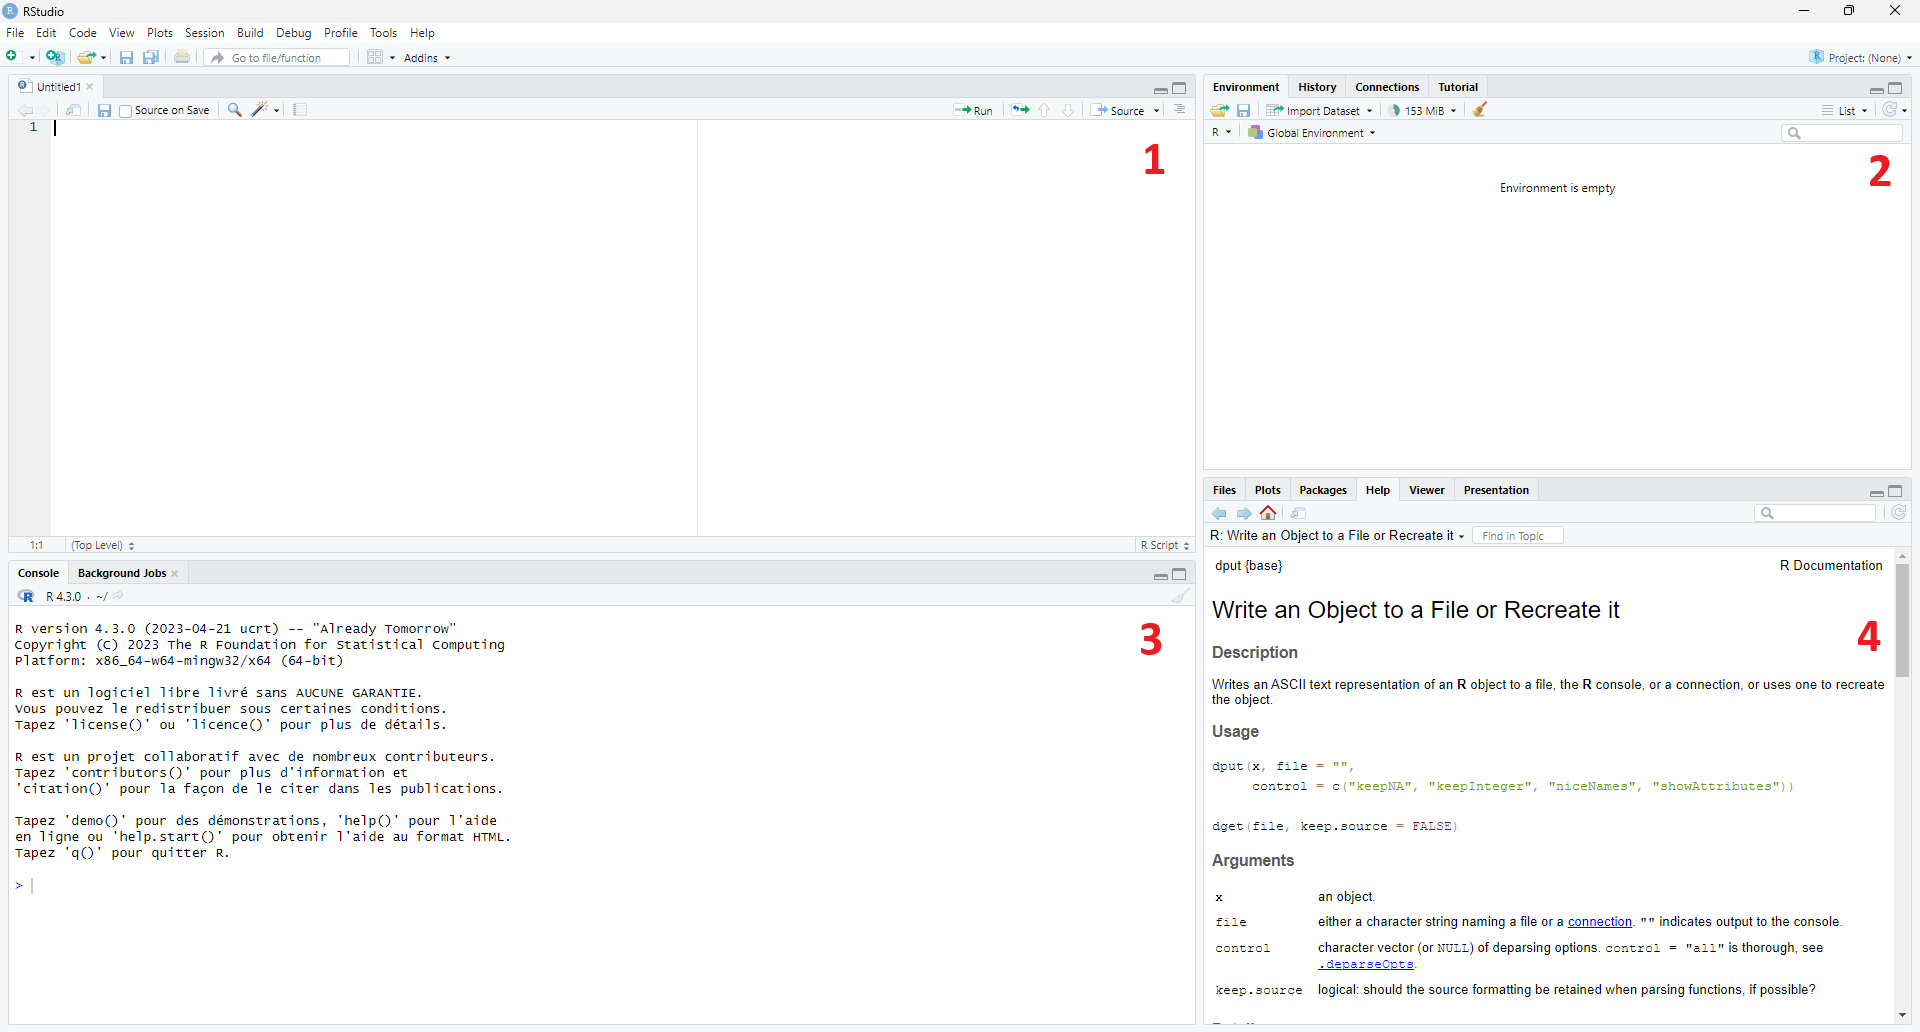
\includegraphics[width=26.67in]{images/environnement}
Chacune des quatre zones a sa propre utilité:

\begin{enumerate}
\def\labelenumi{\arabic{enumi}.}
\tightlist
\item
  Cette zone est dédiée aux fichiers sources. Ce volet permet d'écrire et de sauvegarder les lignes de code. Ce sera la partie la plus utilisée lors de la programmation. Un nouveau script peut être ouvert à partir de l'onglet \texttt{File} en haut à gauche de l'écran, puis \texttt{New\ File} et \texttt{R\ Script}. Chaque script peut être enregistré soit via le même onglet en choisissant \texttt{Save\ As}, soit en utilisant les raccourcis classiques de votre clavier.
\item
  Cette zone fournit des informations sur les objets, les variables et les données en mémoire sous l'onglet \texttt{Environment}.
\item
  La console est affichée en bas à gauche. Cette partie permet d'entrer et d'exécuter des instructions et voir les résultats s'afficher.
\item
  Cette zone permet de naviguer dans le répertoire de travail dans l'onglet \texttt{Files}, d'afficher les graphes réalisés dans l'onglet \texttt{Plots}, d'afficher les extensions/packages disponibles sous l'onglet \texttt{Packages} et également d'afficher l'aide (qui est très complète) sous l'onglet \texttt{Help}.
\end{enumerate}

\chapter{Objets et opérateurs}\label{objets-et-opuxe9rateurs}

\section{Objets dans R}\label{objets-dans-r}

Une variable permet de stocker une valeur ou un objet dans R. De cette façon, il sera possible d'accéder à la valeur ou à l'objet qui est stocké dans la variable.

\begin{Shaded}
\begin{Highlighting}[]
\CommentTok{\# Assignation de la valeur 3 à la variable "ma\_variable"}
\NormalTok{ma\_variable }\OtherTok{\textless{}{-}} \DecValTok{3}
\end{Highlighting}
\end{Shaded}

La ligne de code ci-dessus déclare une variable nommée ``ma\_variable'' et lui assigne la valeur de 3. L'exécution de ce code n'affiche pas de résultat dans la console, mais l'objet nommé ``ma\_variable'' est bien créée et stockée dans l'environnement.

Pour afficher le contenu de la variable, il suffit de taper le nom de celle-ci pour l'afficher dans la console.

\begin{Shaded}
\begin{Highlighting}[]
\CommentTok{\# Affichage du contenu de la variable "ma\_variable"}
\NormalTok{ma\_variable}
\end{Highlighting}
\end{Shaded}

\begin{verbatim}
## [1] 3
\end{verbatim}

De plus, il est également possible d'utiliser la fonction \texttt{print()} qui permet d'afficher la valeur ou l'objet de la variable sélectionnée.

\begin{Shaded}
\begin{Highlighting}[]
\CommentTok{\# Affichage du contenur de la variable "ma\_variable"}
\FunctionTok{print}\NormalTok{(ma\_variable)}
\end{Highlighting}
\end{Shaded}

\begin{verbatim}
## [1] 3
\end{verbatim}

En langage R, il existe différents types d'objets qui peuvent être assignés à des variables comme les scalaires, les vecteurs, les facteurs, les matrices et les bases de données. Ces objets sont présentés dans les points suivants.

\subsection{Scalaire}\label{scalaire}

Un scalaire permet de stocker un objet sous forme de valeur numérique, de chaîne de caractères ou de valeur logique.

\begin{Shaded}
\begin{Highlighting}[]
\CommentTok{\# Scalaire numerique}
\NormalTok{a }\OtherTok{\textless{}{-}} \DecValTok{3}
\NormalTok{a}
\end{Highlighting}
\end{Shaded}

\begin{verbatim}
## [1] 3
\end{verbatim}

Une chaîne de caractères est une suite de caractères qui doit être écrit entre guillemets ('' ``).

\begin{Shaded}
\begin{Highlighting}[]
\CommentTok{\# Scalaire sous forme d\textquotesingle{}une chaine de caractères}
\NormalTok{b }\OtherTok{\textless{}{-}} \StringTok{"Statistique"}
\NormalTok{b}
\end{Highlighting}
\end{Shaded}

\begin{verbatim}
## [1] "Statistique"
\end{verbatim}

Une valeur logique est une quantitée binaire (vrai ou faux). Ces variables s'écrivent \texttt{TRUE} et \texttt{FALSE}. Il est également possible d'utiliser \texttt{T} et \texttt{F} comme abréviations.

\begin{Shaded}
\begin{Highlighting}[]
\CommentTok{\# Scalaire logique}
\NormalTok{c }\OtherTok{\textless{}{-}} \ConstantTok{TRUE}
\NormalTok{c}
\end{Highlighting}
\end{Shaded}

\begin{verbatim}
## [1] TRUE
\end{verbatim}

\begin{Shaded}
\begin{Highlighting}[]
\NormalTok{d }\OtherTok{\textless{}{-}}\NormalTok{ F}
\NormalTok{d  }
\end{Highlighting}
\end{Shaded}

\begin{verbatim}
## [1] FALSE
\end{verbatim}

\subsection{Vecteur}\label{vecteur}

Un vecteur est un objet qui permet de stocker une liste ordonnée d'éléments. Les éléments d'un vecteur doivent être du même type.
Pour pouvoir stocker une information dans un seul objet, il faut utiliser la fonction \texttt{c()} qui permet de combiner les arguments de la fonction.

\begin{Shaded}
\begin{Highlighting}[]
\CommentTok{\# Vecteur numérique}
\NormalTok{a }\OtherTok{\textless{}{-}} \FunctionTok{c}\NormalTok{(}\DecValTok{1}\NormalTok{, }\DecValTok{2}\NormalTok{, }\DecValTok{3}\NormalTok{, }\DecValTok{4}\NormalTok{, }\DecValTok{5}\NormalTok{, }\DecValTok{6}\NormalTok{)}
\NormalTok{a}
\end{Highlighting}
\end{Shaded}

\begin{verbatim}
## [1] 1 2 3 4 5 6
\end{verbatim}

\begin{Shaded}
\begin{Highlighting}[]
\CommentTok{\# Vecteur sous forme d\textquotesingle{}une chaine de caractères}
\NormalTok{b }\OtherTok{\textless{}{-}} \FunctionTok{c}\NormalTok{(}\StringTok{"Un"}\NormalTok{, }\StringTok{"Deux"}\NormalTok{, }\StringTok{"Trois"}\NormalTok{, }\StringTok{"Quatre"}\NormalTok{, }\StringTok{"Cinq"}\NormalTok{, }\StringTok{"Six"}\NormalTok{)}
\NormalTok{b}
\end{Highlighting}
\end{Shaded}

\begin{verbatim}
## [1] "Un"     "Deux"   "Trois"  "Quatre" "Cinq"   "Six"
\end{verbatim}

\begin{Shaded}
\begin{Highlighting}[]
\CommentTok{\# Vecteur logique}
\NormalTok{c }\OtherTok{\textless{}{-}} \FunctionTok{c}\NormalTok{(}\ConstantTok{TRUE}\NormalTok{, }\ConstantTok{FALSE}\NormalTok{, }\ConstantTok{TRUE}\NormalTok{, }\ConstantTok{FALSE}\NormalTok{, }\ConstantTok{FALSE}\NormalTok{, }\ConstantTok{TRUE}\NormalTok{)}
\NormalTok{c}
\end{Highlighting}
\end{Shaded}

\begin{verbatim}
## [1]  TRUE FALSE  TRUE FALSE FALSE  TRUE
\end{verbatim}

Étant donné que le vecteur est un objet ordonné, il est possible d'accéder, remplacer ou modifier un ou plusieurs éléments par rapport à leur position dans l'objet. Il est nécessaire d'utiliser les crochets \texttt{{[}\ {]}} pour indiquer le ou les éléments à manipuler. Afin de connaître la longueur d'un vecteur, il faut utiliser la fonction \texttt{length()}.

\begin{Shaded}
\begin{Highlighting}[]
\CommentTok{\# Vecteur logique}
\FunctionTok{length}\NormalTok{(b)}
\end{Highlighting}
\end{Shaded}

\begin{verbatim}
## [1] 6
\end{verbatim}

\begin{Shaded}
\begin{Highlighting}[]
\FunctionTok{length}\NormalTok{(c)}
\end{Highlighting}
\end{Shaded}

\begin{verbatim}
## [1] 6
\end{verbatim}

Pour accéder un seul élément du vecteur, il suffit d'écrire le nom de la variable suivi de crochets contenant la position de l'élément sélectionné.

\begin{Shaded}
\begin{Highlighting}[]
\CommentTok{\# Extraction d\textquotesingle{}un élément:}
\NormalTok{b[}\DecValTok{2}\NormalTok{]}
\end{Highlighting}
\end{Shaded}

\begin{verbatim}
## [1] "Deux"
\end{verbatim}

Il est possible d'accéder à plusieurs éléments en mettant un vecteur de position entre crochets.

\begin{Shaded}
\begin{Highlighting}[]
\CommentTok{\# Extraction de plusieurs éléments:}
\NormalTok{b[}\FunctionTok{c}\NormalTok{(}\DecValTok{2}\NormalTok{,}\DecValTok{3}\NormalTok{,}\DecValTok{5}\NormalTok{)]}
\end{Highlighting}
\end{Shaded}

\begin{verbatim}
## [1] "Deux"  "Trois" "Cinq"
\end{verbatim}

Il est aussi possible d'accéder à une série d'éléments à la suite en mettant le signe \texttt{:} entre les 2 positions désirées.

\begin{Shaded}
\begin{Highlighting}[]
\CommentTok{\# Extraction d\textquotesingle{}une série d\textquotesingle{}éléments:}
\NormalTok{b[}\DecValTok{2}\SpecialCharTok{:}\DecValTok{5}\NormalTok{]}
\end{Highlighting}
\end{Shaded}

\begin{verbatim}
## [1] "Deux"   "Trois"  "Quatre" "Cinq"
\end{verbatim}

Il est également possible d'accéder à certaines lignes en fonction de la valeur logique d'un vecteur ayant la même taille du vecteur sélectionné. Si la position est mise à \texttt{TRUE}, la valeur sera sélectionnée et dans le cas dans lequel la valeur est mise à \texttt{FALSE} la valeur ne sera pas retenue.

\begin{Shaded}
\begin{Highlighting}[]
\CommentTok{\# Extraction de plusieurs éléments en fontion de la valeur logique:}
\NormalTok{b[}\FunctionTok{c}\NormalTok{(}\ConstantTok{FALSE}\NormalTok{, }\ConstantTok{TRUE}\NormalTok{, }\ConstantTok{TRUE}\NormalTok{, }\ConstantTok{FALSE}\NormalTok{, }\ConstantTok{TRUE}\NormalTok{, }\ConstantTok{TRUE}\NormalTok{)]}
\end{Highlighting}
\end{Shaded}

\begin{verbatim}
## [1] "Deux"  "Trois" "Cinq"  "Six"
\end{verbatim}

Il est également possible de créer un vecteur vide dans lequel il sera par la suite possible d'ajouter des valeurs. Le code qui suit permet de créer ce vecteur:

\begin{Shaded}
\begin{Highlighting}[]
\NormalTok{vide }\OtherTok{\textless{}{-}} \FunctionTok{vector}\NormalTok{()}
\end{Highlighting}
\end{Shaded}

\subsection{Facteur}\label{facteur}

Un facteur est un vecteur dont les éléments peuvent prendre que des valeurs prédéfinies. Un facteur dispose de l'argument \texttt{levels} qui permet de définir des catégories de valeurs. Le facteur est généralement utilisé pour stocker des variables catégorielles.

Pour commencer, il faut définir un vecteur qui peut être numérique, logique ou chaine de caractères. Le facteur est une variable nominale.

\begin{Shaded}
\begin{Highlighting}[]
\NormalTok{genre }\OtherTok{\textless{}{-}} \FunctionTok{c}\NormalTok{(}\StringTok{"Homme"}\NormalTok{, }\StringTok{"Femme"}\NormalTok{, }\StringTok{"Femme"}\NormalTok{, }\StringTok{"Femme"}\NormalTok{, }\StringTok{"Homme"}\NormalTok{)}
\NormalTok{genre}
\end{Highlighting}
\end{Shaded}

\begin{verbatim}
## [1] "Homme" "Femme" "Femme" "Femme" "Homme"
\end{verbatim}

La fonction \texttt{factor()} permet de créer un facteur à partir d'un vecteur.

\begin{Shaded}
\begin{Highlighting}[]
\NormalTok{genre }\OtherTok{\textless{}{-}} \FunctionTok{factor}\NormalTok{(genre)}
\NormalTok{genre}
\end{Highlighting}
\end{Shaded}

\begin{verbatim}
## [1] Homme Femme Femme Femme Homme
## Levels: Femme Homme
\end{verbatim}

On note que la sortie est légèrement différente lorsque le vecteur est mis sous forme de facteur à 2 niveaux (Femme, Homme). Ceci s'affiche à la ligne \texttt{Levels}. Par défaut, les niveaux d'un facteur sont affichés par ordre alphabétique et numérique croissant. Il est possible de fixer l'ordre en ajoutant l'argument \texttt{levels} en appliquant la fonction \texttt{factor()}.

\begin{Shaded}
\begin{Highlighting}[]
\NormalTok{sexe }\OtherTok{\textless{}{-}} \FunctionTok{c}\NormalTok{(}\StringTok{"H"}\NormalTok{, }\StringTok{"F"}\NormalTok{, }\StringTok{"F"}\NormalTok{, }\StringTok{"F"}\NormalTok{, }\StringTok{"H"}\NormalTok{)}
\NormalTok{sexe }\OtherTok{\textless{}{-}} \FunctionTok{factor}\NormalTok{(sexe, }\AttributeTok{levels =} \FunctionTok{c}\NormalTok{(}\StringTok{"H"}\NormalTok{, }\StringTok{"F"}\NormalTok{))}
\NormalTok{sexe}
\end{Highlighting}
\end{Shaded}

\begin{verbatim}
## [1] H F F F H
## Levels: H F
\end{verbatim}

Dans le cas dans lequel on aimerait modifier un élément, il n'est pas possible d'affecter une valeur qui n'est pas défini comme un niveau. On voit donc apparaître une erreur dans la console.

\begin{Shaded}
\begin{Highlighting}[]
\NormalTok{genre[}\DecValTok{2}\NormalTok{] }\OtherTok{\textless{}{-}} \StringTok{"Fille"}
\end{Highlighting}
\end{Shaded}

\begin{verbatim}
## Warning in `[<-.factor`(`*tmp*`, 2, value = "Fille"): niveau de facteur
## incorrect, NAs générés
\end{verbatim}

Il est possible de renommer les niveaux en utilisant la fonction \texttt{levels()}. \textbf{Il faut faire attention à l'ordre lorsqu'on utilise la fonction \texttt{levels()}.} L'argument \texttt{order} permet d'ordonner les labels proposés. Le facteur est dès lors une variable ordinale.

\begin{Shaded}
\begin{Highlighting}[]
\FunctionTok{levels}\NormalTok{(genre) }\OtherTok{\textless{}{-}} \FunctionTok{c}\NormalTok{(}\StringTok{"Fille"}\NormalTok{, }\StringTok{"Garcon"}\NormalTok{)}
\NormalTok{genre}
\end{Highlighting}
\end{Shaded}

\begin{verbatim}
## [1] Garcon <NA>   Fille  Fille  Garcon
## Levels: Fille Garcon
\end{verbatim}

Il est possible d'avoir un facteur numérique en y affectant une catégorie avec l'argument \texttt{labels} lors de l'utilisation de la fonction \texttt{factor()}.

\begin{Shaded}
\begin{Highlighting}[]
\NormalTok{satisfaction }\OtherTok{\textless{}{-}} \FunctionTok{factor}\NormalTok{(}\FunctionTok{c}\NormalTok{(}\DecValTok{3}\NormalTok{, }\DecValTok{3}\NormalTok{, }\DecValTok{4}\NormalTok{, }\DecValTok{1}\NormalTok{, }\DecValTok{2}\NormalTok{, }\DecValTok{1}\NormalTok{, }\DecValTok{1}\NormalTok{), }
                       \AttributeTok{labels =} \FunctionTok{c}\NormalTok{(}\StringTok{"Pas du tout d\textquotesingle{}accord"}\NormalTok{, }\StringTok{"Pas d\textquotesingle{}accord"}\NormalTok{, }
                                  \StringTok{"D\textquotesingle{}accord"}\NormalTok{, }\StringTok{"Tout à fait d\textquotesingle{}accord"}\NormalTok{), }
                       \AttributeTok{order =} \ConstantTok{TRUE}\NormalTok{)}
\NormalTok{satisfaction}
\end{Highlighting}
\end{Shaded}

\begin{verbatim}
## [1] D'accord             D'accord             Tout à fait d'accord
## [4] Pas du tout d'accord Pas d'accord         Pas du tout d'accord
## [7] Pas du tout d'accord
## 4 Levels: Pas du tout d'accord < Pas d'accord < ... < Tout à fait d'accord
\end{verbatim}

\subsection{Matrice}\label{matrice}

Une matrice est un vecteur dont les éléments sont disposés sous forme d'un tableau qui comporte des lignes et des colonnes. De façon équivalente au vecteur, les éléments de la matrices doivent être de même classe (numérique, logique ou chaîne de caractères). La fonction \texttt{matrix()} permet de déclarer une matrice. Il faut ajouter l'argument \texttt{ncol} et/ou \texttt{nrow} pour déterminer la forme de la matrice.

\begin{Shaded}
\begin{Highlighting}[]
\NormalTok{A }\OtherTok{\textless{}{-}} \FunctionTok{matrix}\NormalTok{(}\DecValTok{1}\SpecialCharTok{:}\DecValTok{24}\NormalTok{, }\AttributeTok{nrow=}\DecValTok{6}\NormalTok{, }\AttributeTok{ncol=}\DecValTok{4}\NormalTok{, }\AttributeTok{byrow=}\ConstantTok{FALSE}\NormalTok{)}
\NormalTok{A}
\end{Highlighting}
\end{Shaded}

\begin{verbatim}
##      [,1] [,2] [,3] [,4]
## [1,]    1    7   13   19
## [2,]    2    8   14   20
## [3,]    3    9   15   21
## [4,]    4   10   16   22
## [5,]    5   11   17   23
## [6,]    6   12   18   24
\end{verbatim}

Par défaut, le remplissage se fait par colonne. Il faut donc mettre l'argument \texttt{byrow} à \texttt{TRUE} pour remplir la matrice par ligne.

\begin{Shaded}
\begin{Highlighting}[]
\NormalTok{B }\OtherTok{\textless{}{-}} \FunctionTok{matrix}\NormalTok{(}\DecValTok{1}\SpecialCharTok{:}\DecValTok{24}\NormalTok{, }\AttributeTok{nrow=}\DecValTok{6}\NormalTok{, }\AttributeTok{ncol=}\DecValTok{4}\NormalTok{, }\AttributeTok{byrow=}\ConstantTok{TRUE}\NormalTok{)}
\NormalTok{B}
\end{Highlighting}
\end{Shaded}

\begin{verbatim}
##      [,1] [,2] [,3] [,4]
## [1,]    1    2    3    4
## [2,]    5    6    7    8
## [3,]    9   10   11   12
## [4,]   13   14   15   16
## [5,]   17   18   19   20
## [6,]   21   22   23   24
\end{verbatim}

L'objet matrice dispose de la fonction \texttt{dim()} qui permet d'obtenir sa dimension. Le premier terme correspond aux nombres de lignes et le deuxième correspond aux nombres de colonnes.

\begin{Shaded}
\begin{Highlighting}[]
\FunctionTok{dim}\NormalTok{(B)}
\end{Highlighting}
\end{Shaded}

\begin{verbatim}
## [1] 6 4
\end{verbatim}

Les fonctions \texttt{rownames()} et \texttt{colnames()} permettent de récupérer ou de définir les noms des lignes et des colonnes. Attention de bien mettre le bon nombre de noms aux lignes et aux colonnes.

\begin{Shaded}
\begin{Highlighting}[]
\FunctionTok{rownames}\NormalTok{(B) }\OtherTok{\textless{}{-}} \FunctionTok{c}\NormalTok{(}\StringTok{"L1"}\NormalTok{, }\StringTok{"L2"}\NormalTok{, }\StringTok{"L3"}\NormalTok{, }\StringTok{"L4"}\NormalTok{, }\StringTok{"L5"}\NormalTok{, }\StringTok{"L6"}\NormalTok{)}
\FunctionTok{colnames}\NormalTok{(B) }\OtherTok{\textless{}{-}} \FunctionTok{c}\NormalTok{(}\StringTok{"C1"}\NormalTok{, }\StringTok{"C2"}\NormalTok{, }\StringTok{"C3"}\NormalTok{, }\StringTok{"C4"}\NormalTok{)}
\NormalTok{B}
\end{Highlighting}
\end{Shaded}

\begin{verbatim}
##    C1 C2 C3 C4
## L1  1  2  3  4
## L2  5  6  7  8
## L3  9 10 11 12
## L4 13 14 15 16
## L5 17 18 19 20
## L6 21 22 23 24
\end{verbatim}

Comme pour le vecteur, il est possible d'accéder à un ou plusieurs éléments de la matrice.
Pour extraire une ligne de la matrice, il faut utiliser les crochets avec une virgule pour délimiter les deux dimensions de la matrice\texttt{{[}\ ,\ {]}}. Le premier terme (celui avant la virgule) permet d'accéder aux colonnes et le deuxième terme (celui après la virgule) permet d'accéder aux lignes.
Pour accéder à un seul élément, il faut indiquer la position de la ligne et de la colonne désirée.

\begin{Shaded}
\begin{Highlighting}[]
\CommentTok{\# Extraction d\textquotesingle{}un seul élément}
\NormalTok{A[}\DecValTok{2}\NormalTok{,}\DecValTok{3}\NormalTok{]}
\end{Highlighting}
\end{Shaded}

\begin{verbatim}
## [1] 14
\end{verbatim}

Pour accéder à une ligne complète, il suffit de mettre la position de la ligne désirée avant la virgule.

\begin{Shaded}
\begin{Highlighting}[]
\CommentTok{\# Extraction d\textquotesingle{}une ligne}
\NormalTok{A[}\DecValTok{2}\NormalTok{, ]}
\end{Highlighting}
\end{Shaded}

\begin{verbatim}
## [1]  2  8 14 20
\end{verbatim}

Pour accéder à une colonne complète, il suffit de mettre la position de la colonne désirée après la virgule.

\begin{Shaded}
\begin{Highlighting}[]
\CommentTok{\# Extraction d\textquotesingle{}une colonne}
\NormalTok{A[, }\DecValTok{3}\NormalTok{]}
\end{Highlighting}
\end{Shaded}

\begin{verbatim}
## [1] 13 14 15 16 17 18
\end{verbatim}

Pour accéder à un groupe d'élément, il faut déterminer l'intervalle des lignes et des colonnes désirées.

\begin{Shaded}
\begin{Highlighting}[]
\CommentTok{\# Extraction de quelques éléments regroupées}
\NormalTok{A[}\DecValTok{3}\SpecialCharTok{:}\DecValTok{5}\NormalTok{, }\DecValTok{2}\SpecialCharTok{:}\DecValTok{3}\NormalTok{]}
\end{Highlighting}
\end{Shaded}

\begin{verbatim}
##      [,1] [,2]
## [1,]    9   15
## [2,]   10   16
## [3,]   11   17
\end{verbatim}

\subsection{Dataframe}\label{dataframe}

Un jeu de données se structure sous forme d'un tableau dans lequel chaque ligne correspond à une observation (individu) et chaque colonne à une caractéristique (variable). Les data frame sont les objets les plus utilisées lors de l'analyse d'une base de données. Contrairement aux vecteurs et aux matrices, une dataframe peut avoir différents type de variables (numérique, logique et chaînes de caractères). La fonction \texttt{data.frame()} permet la création de la base de données.

\begin{Shaded}
\begin{Highlighting}[]
\NormalTok{dataframe }\OtherTok{\textless{}{-}} \FunctionTok{data.frame}\NormalTok{(}
  \AttributeTok{ID =} \DecValTok{1}\SpecialCharTok{:}\DecValTok{5}\NormalTok{,}
  \AttributeTok{Genre =} \FunctionTok{c}\NormalTok{(}\StringTok{"Homme"}\NormalTok{, }\StringTok{"Femme"}\NormalTok{, }\StringTok{"Femme"}\NormalTok{, }\StringTok{"Femme"}\NormalTok{, }\StringTok{"Homme"}\NormalTok{),}
  \AttributeTok{Age =} \FunctionTok{c}\NormalTok{(}\DecValTok{45}\NormalTok{, }\DecValTok{42}\NormalTok{, }\DecValTok{45}\NormalTok{, }\DecValTok{43}\NormalTok{, }\DecValTok{44}\NormalTok{)}
\NormalTok{)}
\NormalTok{dataframe}
\end{Highlighting}
\end{Shaded}

\begin{verbatim}
##   ID Genre Age
## 1  1 Homme  45
## 2  2 Femme  42
## 3  3 Femme  45
## 4  4 Femme  43
## 5  5 Homme  44
\end{verbatim}

Les colonnes d'une dataframe sont toujours nommées et correspondent à la variable mesurée. Les lignes sont automatiquement numérotées par ordre.

La fonction \texttt{str()} permet d'afficher la structure de la dataframe en affichat le nom de la variable, le type de celle-ci ainsi que les valeurs des observations.

\begin{Shaded}
\begin{Highlighting}[]
\CommentTok{\# Structure}
\FunctionTok{str}\NormalTok{(dataframe)}
\end{Highlighting}
\end{Shaded}

\begin{verbatim}
## 'data.frame':    5 obs. of  3 variables:
##  $ ID   : int  1 2 3 4 5
##  $ Genre: chr  "Homme" "Femme" "Femme" "Femme" ...
##  $ Age  : num  45 42 45 43 44
\end{verbatim}

La fonction \texttt{View()} permet de visionner la data frame dans une autre fenêtre.

\begin{Shaded}
\begin{Highlighting}[]
\CommentTok{\# Structure}
\FunctionTok{View}\NormalTok{(dataframe)}
\end{Highlighting}
\end{Shaded}

Afin d'analyser les données, il est important de pouvoir d'en extraire uniquement une partie. Il existe deux façons d'extraire une colonne. La première consiste à reproduire le cas de la matrice en séléctionnant la position de la colonne.

\begin{Shaded}
\begin{Highlighting}[]
\CommentTok{\# Extraction de colonnes}
\NormalTok{dataframe[, }\DecValTok{2}\NormalTok{]}
\end{Highlighting}
\end{Shaded}

\begin{verbatim}
## [1] "Homme" "Femme" "Femme" "Femme" "Homme"
\end{verbatim}

La deuxième option est d'utiliser le symbole \texttt{\$}. Il doit être placé entre le nom de la data frame et le nom de la colonne.
\textbf{Il est conseillé d'utiliser cette option pour extraire une colonne d'une data frame.}

\begin{Shaded}
\begin{Highlighting}[]
\CommentTok{\# Extraction de colonnes}
\NormalTok{dataframe}\SpecialCharTok{$}\NormalTok{Genre}
\end{Highlighting}
\end{Shaded}

\begin{verbatim}
## [1] "Homme" "Femme" "Femme" "Femme" "Homme"
\end{verbatim}

Pour extraire une ligne de la base de donnée, il faut procéder comme pour la matrice.

\begin{Shaded}
\begin{Highlighting}[]
\CommentTok{\# Extraction de ligne}
\NormalTok{dataframe[}\DecValTok{2}\NormalTok{, ]}
\end{Highlighting}
\end{Shaded}

\begin{verbatim}
##   ID Genre Age
## 2  2 Femme  42
\end{verbatim}

Pour extraire les observations (lignes) qui possèdent certaines caractéristiques, il est possible d'écrire la ligne suivante comme suit:

\begin{Shaded}
\begin{Highlighting}[]
\CommentTok{\# Extraction de ligne}
\NormalTok{dataframe[dataframe}\SpecialCharTok{$}\NormalTok{Genre }\SpecialCharTok{==} \StringTok{"Homme"}\NormalTok{, ]}
\end{Highlighting}
\end{Shaded}

\begin{verbatim}
##   ID Genre Age
## 1  1 Homme  45
## 5  5 Homme  44
\end{verbatim}

Il est également possible de mettre plusieurs conditions.

\begin{Shaded}
\begin{Highlighting}[]
\CommentTok{\# Extraction de ligne}
\NormalTok{dataframe[dataframe}\SpecialCharTok{$}\NormalTok{Genre }\SpecialCharTok{==} \StringTok{"Femme"} \SpecialCharTok{\&}\NormalTok{ dataframe}\SpecialCharTok{$}\NormalTok{Age }\SpecialCharTok{\textless{}} \DecValTok{44}\NormalTok{, ]}
\end{Highlighting}
\end{Shaded}

\begin{verbatim}
##   ID Genre Age
## 2  2 Femme  42
## 4  4 Femme  43
\end{verbatim}

Il est possible d'ajouter une colonne à la base de données. Plusieurs options sont possibles:

\begin{enumerate}
\def\labelenumi{\arabic{enumi}.}
\tightlist
\item
  Créer un vecteur de même taille que la longueur de la base de données et l'ajouter à la base de données en utilisant la fonction \texttt{cbind()}.
\item
  Créer une nouvelle variable directement dans la base de données en déterminant son nom grâce au signe \$.
\end{enumerate}

\begin{Shaded}
\begin{Highlighting}[]
\NormalTok{yeux }\OtherTok{\textless{}{-}} \FunctionTok{c}\NormalTok{(}\StringTok{"brun"}\NormalTok{, }\StringTok{"brun"}\NormalTok{, }\StringTok{"bleu"}\NormalTok{, }\StringTok{"bleu"}\NormalTok{, }\StringTok{"brun"}\NormalTok{)}
\NormalTok{dataframe }\OtherTok{\textless{}{-}} \FunctionTok{cbind}\NormalTok{(dataframe, yeux)}

\NormalTok{dataframe}\SpecialCharTok{$}\NormalTok{cheveux }\OtherTok{\textless{}{-}} \FunctionTok{c}\NormalTok{(}\StringTok{"blond"}\NormalTok{, }\StringTok{"brun"}\NormalTok{, }\StringTok{"blond"}\NormalTok{, }\StringTok{"noir"}\NormalTok{, }\StringTok{"noir"}\NormalTok{)}

\FunctionTok{str}\NormalTok{(dataframe)}
\end{Highlighting}
\end{Shaded}

\begin{verbatim}
## 'data.frame':    5 obs. of  5 variables:
##  $ ID     : int  1 2 3 4 5
##  $ Genre  : chr  "Homme" "Femme" "Femme" "Femme" ...
##  $ Age    : num  45 42 45 43 44
##  $ yeux   : chr  "brun" "brun" "bleu" "bleu" ...
##  $ cheveux: chr  "blond" "brun" "blond" "noir" ...
\end{verbatim}

\section{Opérateurs logiques}\label{opuxe9rateurs-logiques}

\begin{longtable}[]{@{}cl@{}}
\toprule\noalign{}
Opérateur & Description \\
\midrule\noalign{}
\endhead
\bottomrule\noalign{}
\endlastfoot
\textless{} & strictement inférieur \\
\textless= & inférieur ou égal \\
\textgreater{} & strictement supérieur \\
\textgreater= & supérieur ou égal \\
== & égal \\
!= & différent \\
!x & non x \\
x \textbar{} y & x ou y \\
x \& y & x et y \\
\end{longtable}

\chapter{Packages et données}\label{packages-et-donnuxe9es}

Ce premier chapitre introduit deux concepts importants dans R. Le premier est les packages et le second concerne les données.

\section{Installation et gestion des packages}\label{installation-et-gestion-des-packages}

Les packages sont des regroupements de fonctions et de jeux de données développés dans R et qui doivent se télécharger une seule fois, mais ils devront être importés à chaque utilisation. Le code ci-dessous permet d'installer le package ggplot2:

\begin{Shaded}
\begin{Highlighting}[]
\FunctionTok{install.packages}\NormalTok{(}\StringTok{"ggplot2"}\NormalTok{, }\AttributeTok{dependencies =} \ConstantTok{TRUE}\NormalTok{)}
\end{Highlighting}
\end{Shaded}

Avant chaque utilisation des packages, il est nécessaire d'importer le package grâce au code suivant:

\begin{Shaded}
\begin{Highlighting}[]
\FunctionTok{library}\NormalTok{(ggplot2)}
\end{Highlighting}
\end{Shaded}

\section{Téléchargement des données}\label{tuxe9luxe9chargement-des-donnuxe9es}

Dans R, les bases de données se déclinent de plusieurs façons:

\begin{enumerate}
\def\labelenumi{\arabic{enumi}.}
\tightlist
\item
  Les bases de données peuvent être directement incluses dans R ou dans les packages.
\item
  Les bases de données peuvent être créées dans l'environnement sauvées dans l'environnement R. Ces fichiers ont une extension .RData
\item
  Les bases de données peuvent être issues de fichiers externes. Ces fichiers peuvent avoir différentes extensions, les plus courantes étant .csv et .txt.
\end{enumerate}

\subsection{Bases de données issues de la base de R ou des packages}\label{bases-de-donnuxe9es-issues-de-la-base-de-r-ou-des-packages}

Le code suivant permet d'importer le jeu de données ``iris'' disponible de base dans R.

\begin{Shaded}
\begin{Highlighting}[]
\FunctionTok{data}\NormalTok{(iris)}
\end{Highlighting}
\end{Shaded}

Un objet \texttt{iris} apparait dans l'environnement du projet comme le montre la figure suivante.

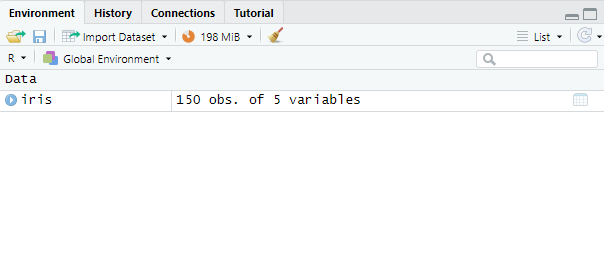
\includegraphics[width=8.39in]{images/environment_forDataDownload}

Si les données sont dans un package, le package doit être importé au préalable.

\subsection{Bases de données issues dans un fichier .RData}\label{bases-de-donnuxe9es-issues-dans-un-fichier-.rdata}

Les fichiers \texttt{.RData} sont spécifique au language R et peuvent contenir plusieurs objets en un seul fichier. Pour importer des données, il faut utiliser la fonction \texttt{load()}

\begin{Shaded}
\begin{Highlighting}[]
\FunctionTok{load}\NormalTok{(}\StringTok{"04{-}data.RData"}\NormalTok{)}
\end{Highlighting}
\end{Shaded}

Tous les objets importés sont chargés dans l'environnement de travail.

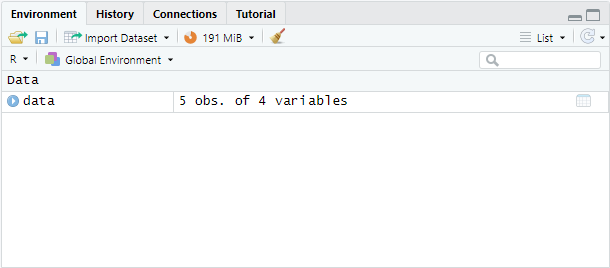
\includegraphics[width=8.47in]{images/environment_forRDataDownload}

\subsection{Bases de données issues de fichiers externes}\label{bases-de-donnuxe9es-issues-de-fichiers-externes}

Les données à analyser sont souvent disponibles dans un fichier externe sous différents formats tels que .csv ou .txt. Pour importer ces données, il existe une fonction par type de fichier (\texttt{read.csv()} et \texttt{read.table()}). Lorsqu'une de ces fonctions est utilisée, le contenu est stocké dans une dataframe. Il est nécessaire de spécifier le chemin d'accès entre votre logiciel et votre fichier à télécharger. Vous pouvez le faire de deux manières: 1. En utilisant la fonction \texttt{setwd()} et en spécifiant à l'intérieur la direction complète qui va permettre au logiciel de retrouver votre document dans vos fichiers. 1. En créant un projet dans lequel vous stockez vos documents. Ces fonctions acceptent des arguments qui permettent de s'adapter à la nature de fichier à importer. Parmi ces arguments, il y en a trois principaux:

\begin{enumerate}
\def\labelenumi{\arabic{enumi}.}
\tightlist
\item
  \texttt{header} qui est une valeur logique (\texttt{TRUE} ou \texttt{FALSE}) pour la présence d'un en-tête avec les noms de variables. Cet argument est mis par défaut à \texttt{TRUE} pour la fonction \texttt{read.csv()} et à \texttt{FALSE} pour la fonction \texttt{read.table()}.
\item
  \texttt{sep} qui est le caractère dont les champs sont séparés. Cet argument est mis par défaut à \texttt{,}.
\item
  \texttt{dec} qui est le séparateur décimal. Cet argument est mis par défaut à \texttt{.}.
\end{enumerate}

Le seul argument obligatoire est le chemin d'accès au fichier à lire. Il n'est pas nécessaire de spécifier le chemin complet si le fichier à lire se trouve dans le dossier du projet. Si ce n'est pas le cas, vous devez spécifier le chemin d'accès complet à partir de ce qui a été fait avec la fonction \texttt{setwd()}. Pour charger une base de donnée nommé \texttt{04-data.csv} dont les valeurs sont séparées par des virgules, il suffit d'écrire la ligne suivante:

\begin{Shaded}
\begin{Highlighting}[]
\NormalTok{csv\_data }\OtherTok{\textless{}{-}} \FunctionTok{read.csv}\NormalTok{(}\StringTok{"04{-}data.csv"}\NormalTok{)}
\NormalTok{csv\_data}
\end{Highlighting}
\end{Shaded}

\begin{verbatim}
##      Nom Age Note.1 Note.2
## 1   Marc  18    5.0   5.50
## 2   Anne  20    6.0   4.00
## 3 Marie   21    4.5   4.75
## 4   Jean  17    3.5   5.00
## 5 Sophie  18    5.0   4.75
\end{verbatim}

Pour charger une base de donnée nommé \texttt{04-data.txt} dont les valeurs sont séparées par des points-virgules, il suffit d'écrire comme dans la ligne suivante en n'oubliant pas de sécifier le caractère de séparation avec l'argument \texttt{sep=";"}.

\begin{Shaded}
\begin{Highlighting}[]
\NormalTok{txt\_data }\OtherTok{\textless{}{-}} \FunctionTok{read.table}\NormalTok{(}\StringTok{"04{-}data.txt"}\NormalTok{, }\AttributeTok{sep =} \StringTok{";"}\NormalTok{, }\AttributeTok{header =} \ConstantTok{TRUE}\NormalTok{)}
\NormalTok{txt\_data}
\end{Highlighting}
\end{Shaded}

\begin{verbatim}
##      Nom Age Note.1 Note.2
## 1   Marc  18    5.0   5.50
## 2   Anne  20    6.0   4.00
## 3  Marie  21    4.5   4.75
## 4   Jean  17    3.5   5.00
## 5 Sophie  18    5.0   4.75
\end{verbatim}

Il est également possible de charger une base de données issues d'un fichier externe en l'important depuis le menu \texttt{File\ \textgreater{}\ Import\ Dataset\ \textgreater{}\ From\ Text} puis de sélectionner le fichier dans vos dossiers.

\chapter{Description des données quantitatives et qualitatives}\label{description-des-donnuxe9es-quantitatives-et-qualitatives}

Ce deuxième chapitre regroupe quelques fonctions pour décrire numériquement et graphiquement les variables quantitatives et qualitatives. Des fonctions spécifiques doivent être utilisées relativement à la nature de la variable.

\begin{Shaded}
\begin{Highlighting}[]
\NormalTok{df }\OtherTok{\textless{}{-}} \FunctionTok{read.csv}\NormalTok{(}\StringTok{"sport.csv"}\NormalTok{, }\AttributeTok{sep =} \StringTok{";"}\NormalTok{, }\AttributeTok{header =} \ConstantTok{TRUE}\NormalTok{)}
\FunctionTok{str}\NormalTok{(df)}
\end{Highlighting}
\end{Shaded}

\begin{verbatim}
## 'data.frame':    15 obs. of  7 variables:
##  $ Identifiant : int  314 323 547 336 678 442 667 890 426 789 ...
##  $ Age         : int  21 17 18 22 29 72 34 28 75 48 ...
##  $ Poids       : num  50.5 46 57.7 52 60 87 66 58.2 89 77 ...
##  $ Grandeur    : int  166 159 170 177 178 182 176 163 179 165 ...
##  $ Satisfaction: chr  "extremement_satisfait" "moyennement_satisfait" "plutot_insatisfait" "pas_du_tout_satisfait" ...
##  $ Sport       : int  180 120 60 30 200 0 180 60 90 320 ...
##  $ Sexe        : chr  "F" "F" "F" "M" ...
\end{verbatim}

On observe qu'il existe plusieurs types de variables.

\section{Description numérique}\label{description-numuxe9rique}

\subsection{Variables qualitatives}\label{variables-qualitatives}

La variable ``Sexe'' est une variable qualitative nominale. Lorsque l'on regarde dans la base de données, on observe qu'elle est considérée comme une chaine de caractères. Il est dès lors possible de la transformer en facteur. Une situation similaire arrive avec la variable ``Satisfaction'' qui est une variable qualitative ordinale. Il est également possible de la transformer afin d'obtenir un facteur ordonné. Pour les deux cas, la transformation s'effectue grâce à la fonction \texttt{factor()}. Lorsque la variable est ordinale, des arguments doivent être ajouté afin de préciser qu'il s'agit d'un facteur ordonné et de donner l'ordre des niveaux.

\begin{Shaded}
\begin{Highlighting}[]
\NormalTok{df}\SpecialCharTok{$}\NormalTok{Sexe }\OtherTok{\textless{}{-}} \FunctionTok{factor}\NormalTok{(df}\SpecialCharTok{$}\NormalTok{Sexe)}
\NormalTok{df}\SpecialCharTok{$}\NormalTok{Sexe}
\end{Highlighting}
\end{Shaded}

\begin{verbatim}
##  [1] F F F M M M M F M F F F F M F
## Levels: F M
\end{verbatim}

\begin{Shaded}
\begin{Highlighting}[]
\NormalTok{df}\SpecialCharTok{$}\NormalTok{Satisfaction }\OtherTok{\textless{}{-}} \FunctionTok{factor}\NormalTok{(df}\SpecialCharTok{$}\NormalTok{Satisfaction, }\AttributeTok{ordered =} \ConstantTok{TRUE}\NormalTok{, }
                          \AttributeTok{levels =} \FunctionTok{c}\NormalTok{(}\StringTok{"pas\_du\_tout\_satisfait"}\NormalTok{, }\StringTok{"plutot\_insatisfait"}\NormalTok{, }
                                     \StringTok{"moyennement\_satisfait"}\NormalTok{, }\StringTok{"tres\_satisfait"}\NormalTok{, }
                                     \StringTok{"extremement\_satisfait"}\NormalTok{))}
\NormalTok{df}\SpecialCharTok{$}\NormalTok{Satisfaction}
\end{Highlighting}
\end{Shaded}

\begin{verbatim}
##  [1] extremement_satisfait moyennement_satisfait plutot_insatisfait   
##  [4] pas_du_tout_satisfait tres_satisfait        pas_du_tout_satisfait
##  [7] moyennement_satisfait plutot_insatisfait    moyennement_satisfait
## [10] tres_satisfait        plutot_insatisfait    pas_du_tout_satisfait
## [13] plutot_insatisfait    tres_satisfait        tres_satisfait       
## 5 Levels: pas_du_tout_satisfait < ... < extremement_satisfait
\end{verbatim}

Pour les variables qualitatives, la description numérique classique est le tableau de contingence que l'on obtient avec la fonction \texttt{table()}. Il est possible de décrire chaque variable à la fois ou de décrire une variable en fonction d'une autre.

\begin{Shaded}
\begin{Highlighting}[]
\FunctionTok{table}\NormalTok{(df}\SpecialCharTok{$}\NormalTok{Sexe)}
\end{Highlighting}
\end{Shaded}

\begin{verbatim}
## 
## F M 
## 9 6
\end{verbatim}

\begin{Shaded}
\begin{Highlighting}[]
\FunctionTok{table}\NormalTok{(df}\SpecialCharTok{$}\NormalTok{Satisfaction)}
\end{Highlighting}
\end{Shaded}

\begin{verbatim}
## 
## pas_du_tout_satisfait    plutot_insatisfait moyennement_satisfait 
##                     3                     4                     3 
##        tres_satisfait extremement_satisfait 
##                     4                     1
\end{verbatim}

\begin{Shaded}
\begin{Highlighting}[]
\FunctionTok{table}\NormalTok{(df}\SpecialCharTok{$}\NormalTok{Sexe, df}\SpecialCharTok{$}\NormalTok{Satisfaction)}
\end{Highlighting}
\end{Shaded}

\begin{verbatim}
##    
##     pas_du_tout_satisfait plutot_insatisfait moyennement_satisfait
##   F                     1                  4                     1
##   M                     2                  0                     2
##    
##     tres_satisfait extremement_satisfait
##   F              2                     1
##   M              2                     0
\end{verbatim}

\subsection{Variables quantitatives}\label{variables-quantitatives}

Les variables quantitatives sont généralement décrites à l'aide de:

\begin{enumerate}
\def\labelenumi{\arabic{enumi}.}
\tightlist
\item
  Mesures de tendance centrale: mode, moyenne, médiane
\item
  Mesures de dispersion: étendue, espace interquartile, variance et écart-type
\end{enumerate}

La moyenne et la médiane peuvent se calculer directement avec les fonctions \texttt{mean()}et \texttt{median()} respectivement. Le mode d'une variable peut s'obtenir en analysant le tableau de contingence. Dans notre cas, on observe qu'il n'y a pas de mode étant donné qu'aucun âge apparaît plusieurs fois.

\begin{Shaded}
\begin{Highlighting}[]
\FunctionTok{mean}\NormalTok{(df}\SpecialCharTok{$}\NormalTok{Age)}
\end{Highlighting}
\end{Shaded}

\begin{verbatim}
## [1] 34.66667
\end{verbatim}

\begin{Shaded}
\begin{Highlighting}[]
\FunctionTok{median}\NormalTok{(df}\SpecialCharTok{$}\NormalTok{Age)}
\end{Highlighting}
\end{Shaded}

\begin{verbatim}
## [1] 29
\end{verbatim}

\begin{Shaded}
\begin{Highlighting}[]
\FunctionTok{table}\NormalTok{(df}\SpecialCharTok{$}\NormalTok{Age)}
\end{Highlighting}
\end{Shaded}

\begin{verbatim}
## 
## 17 18 20 21 22 25 28 29 32 34 35 44 48 72 75 
##  1  1  1  1  1  1  1  1  1  1  1  1  1  1  1
\end{verbatim}

L'étendue d'une variable peut s'obtenir en soustrayant la valeur maximale et la valeur minimale d'une variable. La variance et l'écart-type s'obtiennent directement avec les fonctions \texttt{var()}et \texttt{sd()}respectivement. L'espace interquartile, utilisé pour construire le boxplot, s'obtient grâce à la fonction \texttt{IQR()}.

\begin{Shaded}
\begin{Highlighting}[]
\FunctionTok{min}\NormalTok{(df}\SpecialCharTok{$}\NormalTok{Age)}
\end{Highlighting}
\end{Shaded}

\begin{verbatim}
## [1] 17
\end{verbatim}

\begin{Shaded}
\begin{Highlighting}[]
\FunctionTok{max}\NormalTok{(df}\SpecialCharTok{$}\NormalTok{Age)}
\end{Highlighting}
\end{Shaded}

\begin{verbatim}
## [1] 75
\end{verbatim}

\begin{Shaded}
\begin{Highlighting}[]
\FunctionTok{max}\NormalTok{(df}\SpecialCharTok{$}\NormalTok{Age)}\SpecialCharTok{{-}}\FunctionTok{min}\NormalTok{(df}\SpecialCharTok{$}\NormalTok{Age)}
\end{Highlighting}
\end{Shaded}

\begin{verbatim}
## [1] 58
\end{verbatim}

\begin{Shaded}
\begin{Highlighting}[]
\FunctionTok{var}\NormalTok{(df}\SpecialCharTok{$}\NormalTok{Age)}
\end{Highlighting}
\end{Shaded}

\begin{verbatim}
## [1] 329.6667
\end{verbatim}

\begin{Shaded}
\begin{Highlighting}[]
\FunctionTok{sd}\NormalTok{(df}\SpecialCharTok{$}\NormalTok{Age)}
\end{Highlighting}
\end{Shaded}

\begin{verbatim}
## [1] 18.15673
\end{verbatim}

\begin{Shaded}
\begin{Highlighting}[]
\FunctionTok{IQR}\NormalTok{(df}\SpecialCharTok{$}\NormalTok{Age)}
\end{Highlighting}
\end{Shaded}

\begin{verbatim}
## [1] 18
\end{verbatim}

\section{Description graphique}\label{description-graphique}

\subsection{Variables qualitatives}\label{variables-qualitatives-1}

Les variables qualitatives peuvent être représentées grâce à des graphiques en barre ou des graphiques en camembert. Les fonctions \texttt{barplot()}et \texttt{pie()}permettent de représenter les tableaux de contingence. Pour rappel, il est possible de sauver un objet dans l'environnement et de l'utiliser ensuite directement pour faire les graphes. C'est ce qui est proposé pour le tableau de contigence de la variable ``Satisfaction''.

\begin{Shaded}
\begin{Highlighting}[]
\FunctionTok{barplot}\NormalTok{(}\FunctionTok{table}\NormalTok{(df}\SpecialCharTok{$}\NormalTok{Sexe))}
\end{Highlighting}
\end{Shaded}

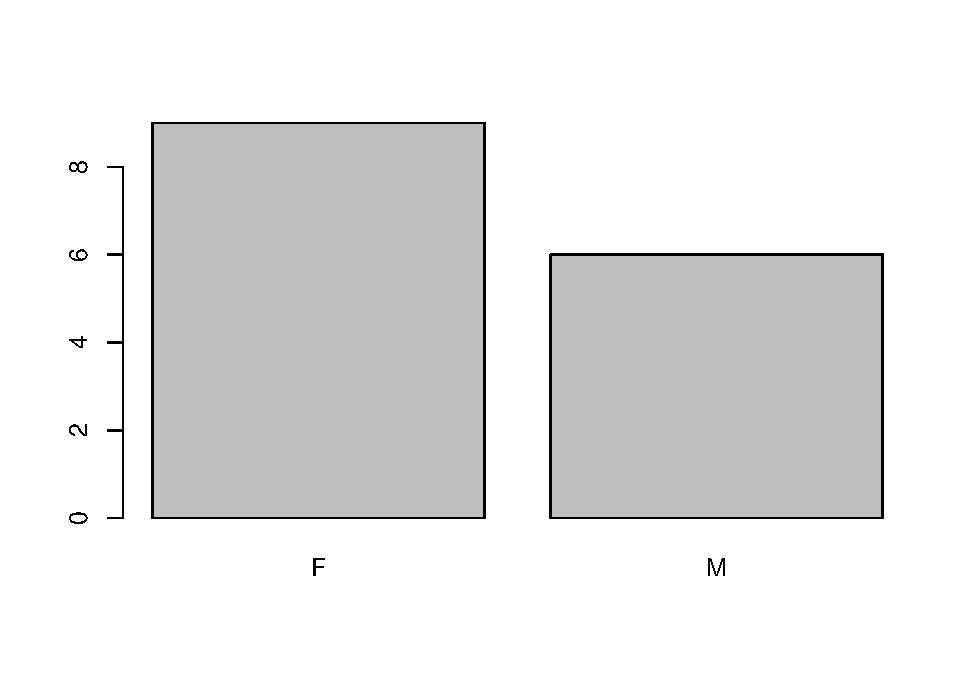
\includegraphics{_main_files/figure-latex/unnamed-chunk-53-1.pdf}

\begin{Shaded}
\begin{Highlighting}[]
\NormalTok{tableSatisfaction }\OtherTok{\textless{}{-}} \FunctionTok{table}\NormalTok{(df}\SpecialCharTok{$}\NormalTok{Satisfaction)}
\FunctionTok{barplot}\NormalTok{(tableSatisfaction)}
\end{Highlighting}
\end{Shaded}

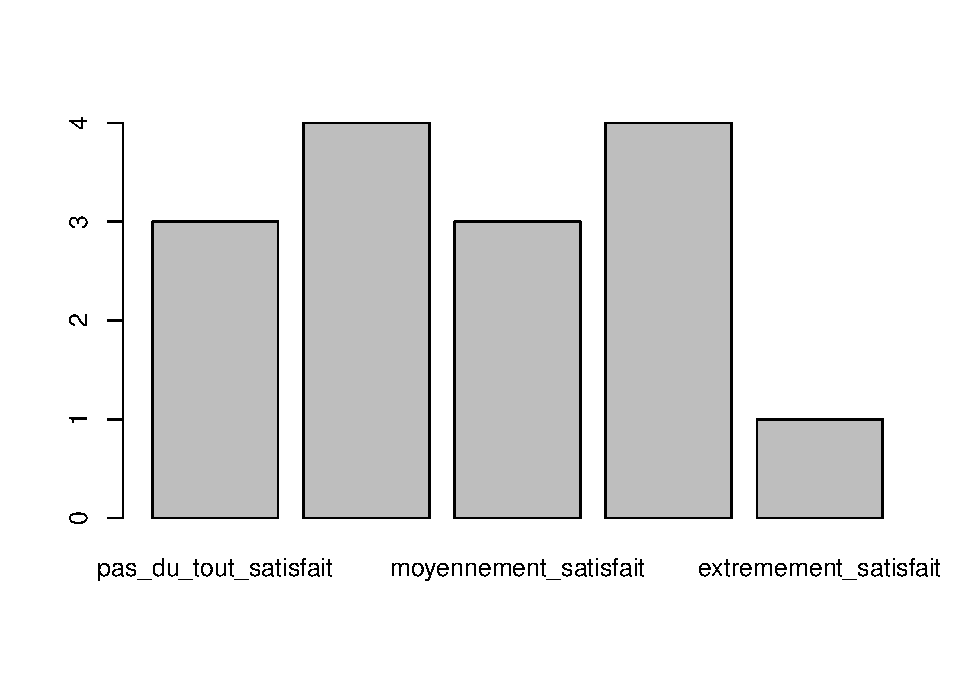
\includegraphics{_main_files/figure-latex/unnamed-chunk-53-2.pdf}

\begin{Shaded}
\begin{Highlighting}[]
\FunctionTok{par}\NormalTok{(}\AttributeTok{mar=}\FunctionTok{c}\NormalTok{(}\DecValTok{11}\NormalTok{,}\DecValTok{4}\NormalTok{,}\DecValTok{4}\NormalTok{,}\DecValTok{4}\NormalTok{))}
\FunctionTok{barplot}\NormalTok{(tableSatisfaction, }\AttributeTok{las=}\DecValTok{2}\NormalTok{)}
\end{Highlighting}
\end{Shaded}

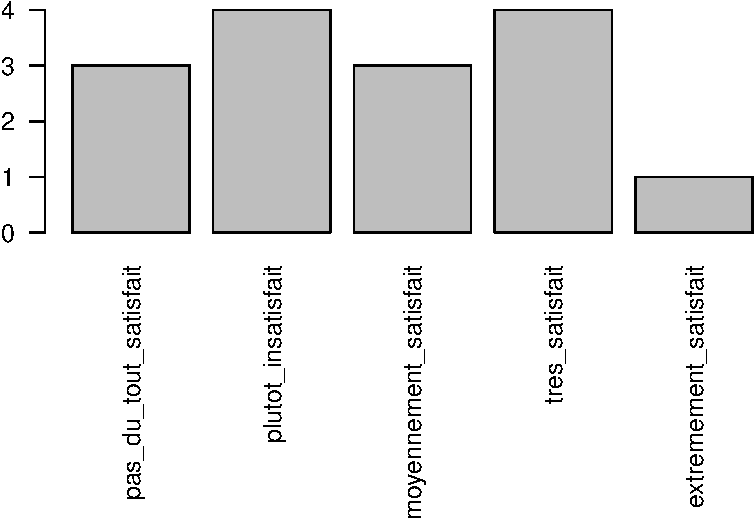
\includegraphics{_main_files/figure-latex/unnamed-chunk-53-3.pdf}

\begin{Shaded}
\begin{Highlighting}[]
\FunctionTok{pie}\NormalTok{(tableSatisfaction)}
\end{Highlighting}
\end{Shaded}

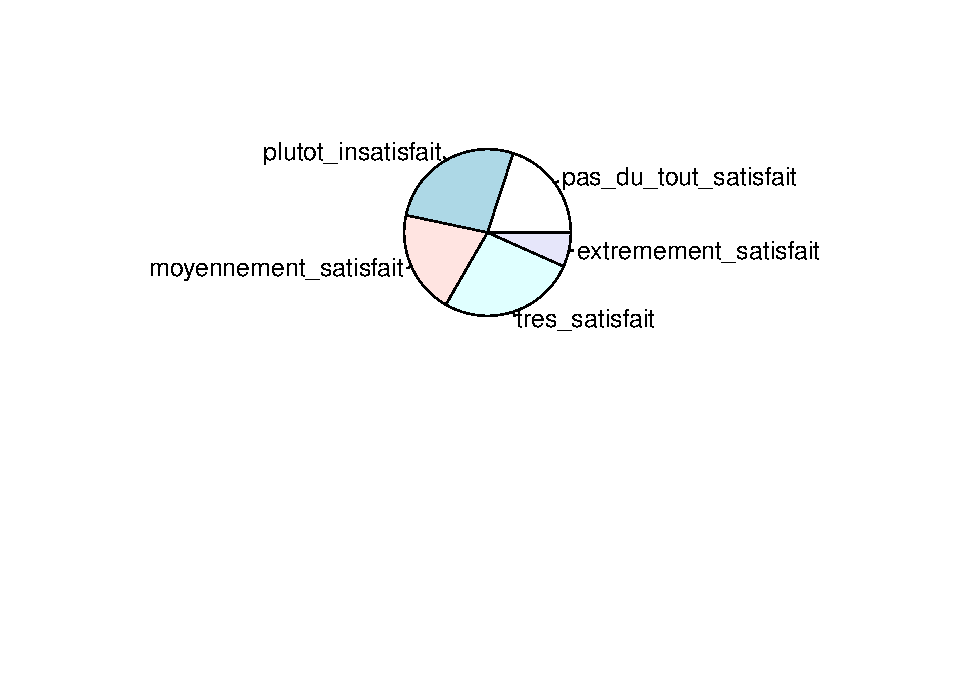
\includegraphics{_main_files/figure-latex/unnamed-chunk-53-4.pdf}

\subsection{Variables quantitatives}\label{variables-quantitatives-1}

Les variables quantitatives peuvent être représentées grâce à des histogrammes ou des boxplots. Les histogrammes permettent de représenter la fréquence de chaque valeur de la variable, tandis que les boxplots représente la distribution de la variable à l'aide des quartiles. Il est possible de spécifier des arguments dans la fonction graphiques afin de donner un titre ou de nomme un axe.

\begin{Shaded}
\begin{Highlighting}[]
\FunctionTok{hist}\NormalTok{(df}\SpecialCharTok{$}\NormalTok{Age, }\AttributeTok{main=}\StringTok{"Histogramme de l\textquotesingle{}age"}\NormalTok{, }\AttributeTok{xlab =} \StringTok{"Age"}\NormalTok{)}
\end{Highlighting}
\end{Shaded}

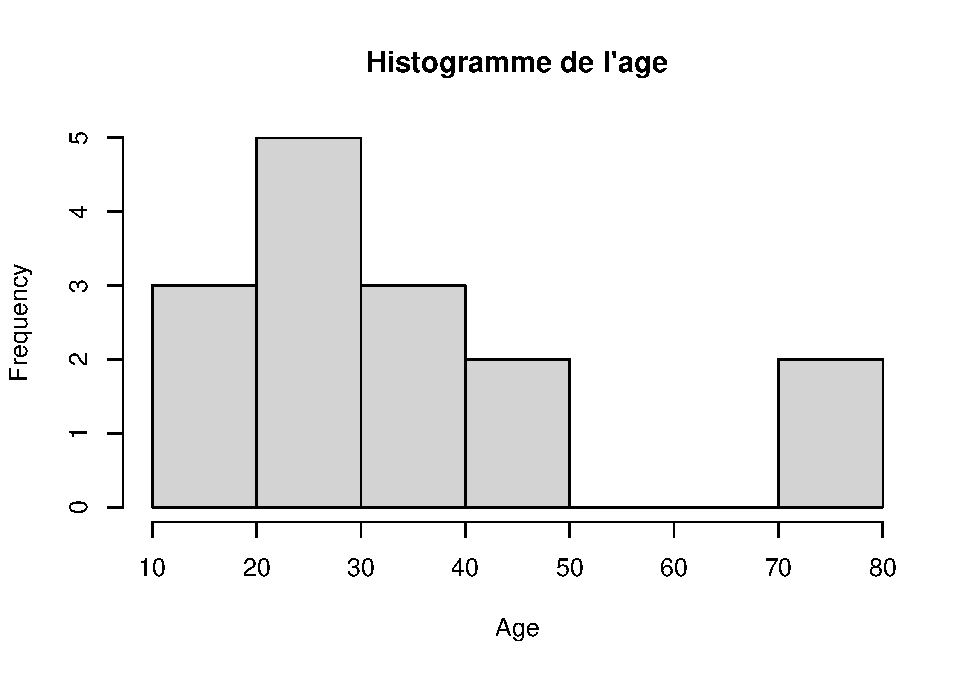
\includegraphics{_main_files/figure-latex/unnamed-chunk-54-1.pdf}

\begin{Shaded}
\begin{Highlighting}[]
\FunctionTok{boxplot}\NormalTok{(df}\SpecialCharTok{$}\NormalTok{Age)}
\end{Highlighting}
\end{Shaded}

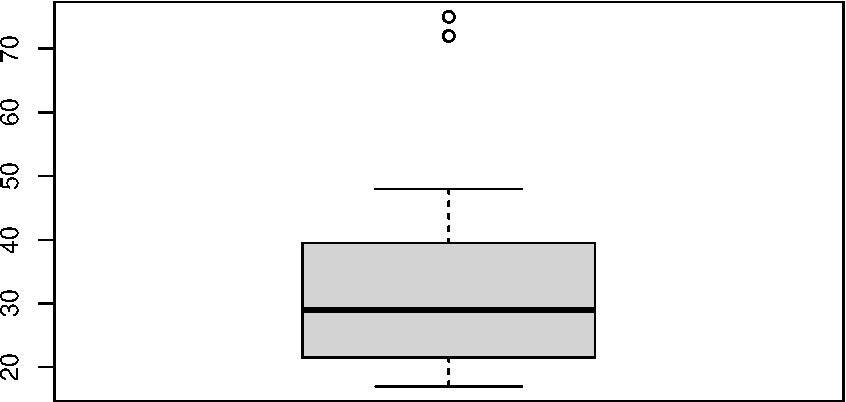
\includegraphics{_main_files/figure-latex/unnamed-chunk-54-2.pdf}

\chapter{Distribution de probabilités}\label{distribution-de-probabilituxe9s}

Ce chapitre couvre les fonctions relatives aux distributions de probabilité. Pour rappel, chaque variable aléatoire a une distribution de probabilité.

Dans ce cours, plusieurs distributions sont abordées, mais la principale est la distribution normale.

\section{Distribution normale}\label{distribution-normale}

La distribution normale est caractérisée par deux paramètres, la moyenne et l'écart-type. La variation de ces deux paramètres implique que plusieurs distributions normales existent. Lorsque la moyenne vaut 0 et l'écart-type 1, on parle de distribution normale centrée-réduite. Il s'agit de la distribution normale avec laquelle il est commun de travailler.

Plusieurs fonctions existent pour travailler avec la distribution normale: \texttt{dnorm()}, \texttt{pnorm()}, \texttt{qnorm()}, et \texttt{rnorm()}.

La fonction \texttt{dnorm()} permet de calculer la densité pour n'importe quelle valeur de x. Par exemple, calculons la densité pour une valeur de 3 avec une distribution normale avec les paramètres de moyenne de 4, et d'écart-type de 2. Calculons ensuite la même densité mais pour une distribution normale centrée-réduite. Pour ce cas, on remarque que les résultats sont similaires lorsque les paramètres sont spécifiés et lorsqu'ils ne le sont pas. Ceci s'explique par le fait que les paramètres de la distribution normale centrée-réduite sont les paramètres par défaut de la fonction.

\begin{Shaded}
\begin{Highlighting}[]
\NormalTok{x }\OtherTok{\textless{}{-}} \DecValTok{3}
\FunctionTok{dnorm}\NormalTok{(x, }\AttributeTok{mean =} \DecValTok{4}\NormalTok{, }\AttributeTok{sd =} \DecValTok{2}\NormalTok{)}
\end{Highlighting}
\end{Shaded}

\begin{verbatim}
## [1] 0.1760327
\end{verbatim}

\begin{Shaded}
\begin{Highlighting}[]
\FunctionTok{dnorm}\NormalTok{(x, }\AttributeTok{mean =} \DecValTok{0}\NormalTok{, }\AttributeTok{sd =} \DecValTok{1}\NormalTok{)}
\end{Highlighting}
\end{Shaded}

\begin{verbatim}
## [1] 0.004431848
\end{verbatim}

\begin{Shaded}
\begin{Highlighting}[]
\FunctionTok{dnorm}\NormalTok{(x)}
\end{Highlighting}
\end{Shaded}

\begin{verbatim}
## [1] 0.004431848
\end{verbatim}

Il est également possible de calculer la densité entre deux valeurs. Calculons la densité entre -4 et 4 pour une distribution normale avec une moyenne de 3 et un écart-type de 2.

\begin{Shaded}
\begin{Highlighting}[]
\NormalTok{x }\OtherTok{\textless{}{-}} \FunctionTok{seq}\NormalTok{(}\SpecialCharTok{{-}}\DecValTok{4}\NormalTok{, }\DecValTok{4}\NormalTok{, }\AttributeTok{by=}\DecValTok{1}\NormalTok{)}
\NormalTok{x}
\end{Highlighting}
\end{Shaded}

\begin{verbatim}
## [1] -4 -3 -2 -1  0  1  2  3  4
\end{verbatim}

\begin{Shaded}
\begin{Highlighting}[]
\FunctionTok{dnorm}\NormalTok{(x, }\AttributeTok{mean =} \DecValTok{3}\NormalTok{, }\AttributeTok{sd =} \DecValTok{2}\NormalTok{)}
\end{Highlighting}
\end{Shaded}

\begin{verbatim}
## [1] 0.0004363413 0.0022159242 0.0087641502 0.0269954833 0.0647587978
## [6] 0.1209853623 0.1760326634 0.1994711402 0.1760326634
\end{verbatim}

\begin{Shaded}
\begin{Highlighting}[]
\FunctionTok{sum}\NormalTok{(}\FunctionTok{dnorm}\NormalTok{(x, }\AttributeTok{mean =} \DecValTok{3}\NormalTok{, }\AttributeTok{sd =}\DecValTok{2}\NormalTok{))}
\end{Highlighting}
\end{Shaded}

\begin{verbatim}
## [1] 0.7756925
\end{verbatim}

La fonction \texttt{pnorm} donne la fonction de distribution de la loi normale. La fonction de distribution cumulative (CDF) correspond à la probabilité que la variable X prenne une valeur inférieure ou égale à x. La fonction de survie correspond à la probabilité que la variable X prenne une valeur supérieure à x. La fonction \texttt{pnorm} permet de calculer ces deux fonctions en manipulant le paramètre \texttt{lower.tail}. Lorsque \texttt{lower.tail\ =\ TRUE}, ce qui est le paramètre par défaut, la CDF est obtenue. Lorsque \texttt{lower.tail\ =\ FALSE}, la fonction de survie est obtenue. Prenons le quantile 1 pour une loi normale centrée-réduite et calculons ces deux fonctions.

\begin{Shaded}
\begin{Highlighting}[]
\FunctionTok{pnorm}\NormalTok{(}\DecValTok{1}\NormalTok{, }\AttributeTok{mean =} \DecValTok{0}\NormalTok{, }\AttributeTok{sd =} \DecValTok{1}\NormalTok{)}
\end{Highlighting}
\end{Shaded}

\begin{verbatim}
## [1] 0.8413447
\end{verbatim}

\begin{Shaded}
\begin{Highlighting}[]
\FunctionTok{pnorm}\NormalTok{(}\DecValTok{1}\NormalTok{, }\AttributeTok{mean =} \DecValTok{0}\NormalTok{, }\AttributeTok{sd =} \DecValTok{1}\NormalTok{, }\AttributeTok{lower.tail =} \ConstantTok{FALSE}\NormalTok{)}
\end{Highlighting}
\end{Shaded}

\begin{verbatim}
## [1] 0.1586553
\end{verbatim}

\begin{Shaded}
\begin{Highlighting}[]
\FunctionTok{pnorm}\NormalTok{(}\DecValTok{1}\NormalTok{, }\AttributeTok{mean =} \DecValTok{0}\NormalTok{, }\AttributeTok{sd =} \DecValTok{1}\NormalTok{) }\SpecialCharTok{+} \FunctionTok{pnorm}\NormalTok{(}\DecValTok{1}\NormalTok{, }\AttributeTok{mean =} \DecValTok{0}\NormalTok{, }\AttributeTok{sd =} \DecValTok{1}\NormalTok{, }\AttributeTok{lower.tail =} \ConstantTok{FALSE}\NormalTok{)}
\end{Highlighting}
\end{Shaded}

\begin{verbatim}
## [1] 1
\end{verbatim}

Si nous sommons la probabilité d'être plus petit qu'un quantile donné et la probabilité d'être plus grand que ce même quantile, le résultat est de 1 parce que tout l'espace possible de la distribution est couvert.

\begin{Shaded}
\begin{Highlighting}[]
\FunctionTok{pnorm}\NormalTok{(}\DecValTok{1}\NormalTok{, }\AttributeTok{mean =} \DecValTok{0}\NormalTok{, }\AttributeTok{sd =} \DecValTok{1}\NormalTok{) }\SpecialCharTok{+} \FunctionTok{pnorm}\NormalTok{(}\DecValTok{1}\NormalTok{, }\AttributeTok{mean =} \DecValTok{0}\NormalTok{, }\AttributeTok{sd =} \DecValTok{1}\NormalTok{, }\AttributeTok{lower.tail =} \ConstantTok{FALSE}\NormalTok{)}
\end{Highlighting}
\end{Shaded}

\begin{verbatim}
## [1] 1
\end{verbatim}

Comme la distribution normale centrée-réduite est symmétrique en 0, la CDF est partagée en deux autour de cette valeur.

\begin{Shaded}
\begin{Highlighting}[]
\FunctionTok{pnorm}\NormalTok{(}\DecValTok{0}\NormalTok{, }\AttributeTok{mean =} \DecValTok{0}\NormalTok{, }\AttributeTok{sd =} \DecValTok{1}\NormalTok{) }
\end{Highlighting}
\end{Shaded}

\begin{verbatim}
## [1] 0.5
\end{verbatim}

\begin{Shaded}
\begin{Highlighting}[]
\FunctionTok{pnorm}\NormalTok{(}\DecValTok{0}\NormalTok{, }\AttributeTok{mean =} \DecValTok{0}\NormalTok{, }\AttributeTok{sd =} \DecValTok{1}\NormalTok{, }\AttributeTok{lower.tail =} \ConstantTok{FALSE}\NormalTok{)}
\end{Highlighting}
\end{Shaded}

\begin{verbatim}
## [1] 0.5
\end{verbatim}

La fonction \texttt{qnorm} permet d'obtenir le quantile pour n'importe quelle probabilité. Pour rappel, un quantile est une valeur qui divise les données d'une distribution en segments de même fréquence. Dans le cadre d'une fonction de distribution, il indique la valeur en dessous de laquelle une certaine proportion des données se situe. Cette fonction calcule l'inverse de la fonction \texttt{pnorm}. Pour simplifier la compréhension, reprenons le dernier exemple présenté.

\begin{Shaded}
\begin{Highlighting}[]
\FunctionTok{pnorm}\NormalTok{(}\DecValTok{0}\NormalTok{, }\AttributeTok{mean =} \DecValTok{0}\NormalTok{, }\AttributeTok{sd =} \DecValTok{1}\NormalTok{) }
\end{Highlighting}
\end{Shaded}

\begin{verbatim}
## [1] 0.5
\end{verbatim}

\begin{Shaded}
\begin{Highlighting}[]
\FunctionTok{qnorm}\NormalTok{(}\FloatTok{0.5}\NormalTok{, }\AttributeTok{mean =} \DecValTok{0}\NormalTok{, }\AttributeTok{sd =} \DecValTok{1}\NormalTok{)}
\end{Highlighting}
\end{Shaded}

\begin{verbatim}
## [1] 0
\end{verbatim}

La fonction \texttt{qnorm} permet de retrouver la valeur correspondant à une probabilité, alors que la fonction \texttt{pnorm} permet de calculer la probabilité à partir d'une valeur.

La fonction \texttt{rnorm} permet de générer \(n\) observations à partir d'une distribution normale. Il s'agit d'une fonction particulièrement utilisée pour la simulation. Comme les autres fonctions concernant la distribution normale, les paramètres de base simuler des données avec une moyenne de 0 et un écart-type de 1. Il est possible de modifier ces paramètres comme suit:

\begin{Shaded}
\begin{Highlighting}[]
\FunctionTok{set.seed}\NormalTok{(}\DecValTok{1234}\NormalTok{) }\CommentTok{\#permet de garantir la reproductibilité des analyses }
\FunctionTok{rnorm}\NormalTok{(}\DecValTok{100}\NormalTok{) }
\end{Highlighting}
\end{Shaded}

\begin{verbatim}
##   [1] -1.207065749  0.277429242  1.084441177 -2.345697703  0.429124689
##   [6]  0.506055892 -0.574739960 -0.546631856 -0.564451999 -0.890037829
##  [11] -0.477192700 -0.998386445 -0.776253895  0.064458817  0.959494059
##  [16] -0.110285494 -0.511009506 -0.911195417 -0.837171680  2.415835178
##  [21]  0.134088220 -0.490685897 -0.440547872  0.459589441 -0.693720247
##  [26] -1.448204910  0.574755721 -1.023655723 -0.015138300 -0.935948601
##  [31]  1.102297546 -0.475593079 -0.709440038 -0.501258061 -1.629093469
##  [36] -1.167619262 -2.180039649 -1.340993192 -0.294293859 -0.465897540
##  [41]  1.449496265 -1.068642724 -0.855364634 -0.280623002 -0.994340076
##  [46] -0.968514318 -1.107318193 -1.251985886 -0.523828119 -0.496849957
##  [51] -1.806031257 -0.582075925 -1.108889624 -1.014962009 -0.162309524
##  [56]  0.563055819  1.647817473 -0.773353424  1.605909629 -1.157808548
##  [61]  0.656588464  2.548991071 -0.034760390 -0.669633580 -0.007604756
##  [66]  1.777084448 -1.138607737  1.367827179  1.329564791  0.336472797
##  [71]  0.006892838 -0.455468738 -0.366523933  0.648286568  2.070270861
##  [76] -0.153398412 -1.390700947 -0.723581777  0.258261762 -0.317059115
##  [81] -0.177789958 -0.169994077 -1.372301886 -0.173787170  0.850232257
##  [86]  0.697608712  0.549997351 -0.402731975 -0.191593770 -1.194527880
##  [91] -0.053158819  0.255196001  1.705964007  1.001513252 -0.495583443
##  [96]  0.355550297 -1.134608044  0.878203627  0.972916753  2.121117105
\end{verbatim}

Comme les autres fonctions concernant la distribution normale, les paramètres de base simuler des données avec une moyenne de 0 et un écart-type de 1. Il est possible de modifier ces paramètres comme suit par exemple:

\begin{Shaded}
\begin{Highlighting}[]
\FunctionTok{set.seed}\NormalTok{(}\DecValTok{1234}\NormalTok{)  }
\FunctionTok{rnorm}\NormalTok{(}\DecValTok{100}\NormalTok{, }\AttributeTok{mean =} \DecValTok{3}\NormalTok{, }\AttributeTok{sd =} \FloatTok{1.5}\NormalTok{) }
\end{Highlighting}
\end{Shaded}

\begin{verbatim}
##   [1]  1.1894014  3.4161439  4.6266618 -0.5185466  3.6436870  3.7590838
##   [7]  2.1378901  2.1800522  2.1533220  1.6649433  2.2842110  1.5024203
##  [13]  1.8356192  3.0966882  4.4392411  2.8345718  2.2334857  1.6332069
##  [19]  1.7442425  6.6237528  3.2011323  2.2639712  2.3391782  3.6893842
##  [25]  1.9594196  0.8276926  3.8621336  1.4645164  2.9772925  1.5960771
##  [31]  4.6534463  2.2866104  1.9358399  2.2481129  0.5563598  1.2485711
##  [37] -0.2700595  0.9885102  2.5585592  2.3011537  5.1742444  1.3970359
##  [43]  1.7169530  2.5790655  1.5084899  1.5472285  1.3390227  1.1220212
##  [49]  2.2142578  2.2547251  0.2909531  2.1268861  1.3366656  1.4775570
##  [55]  2.7565357  3.8445837  5.4717262  1.8399699  5.4088644  1.2632872
##  [61]  3.9848827  6.8234866  2.9478594  1.9955496  2.9885929  5.6656267
##  [67]  1.2920884  5.0517408  4.9943472  3.5047092  3.0103393  2.3167969
##  [73]  2.4502141  3.9724299  6.1054063  2.7699024  0.9139486  1.9146273
##  [79]  3.3873926  2.5244113  2.7333151  2.7450089  0.9415472  2.7393192
##  [85]  4.2753484  4.0464131  3.8249960  2.3959020  2.7126093  1.2082082
##  [91]  2.9202618  3.3827940  5.5589460  4.5022699  2.2566248  3.5333254
##  [97]  1.2980879  4.3173054  4.4593751  6.1816757
\end{verbatim}

\section{Distribution de Student}\label{distribution-de-student}

La distribution de Student est une distribution de probabilité utilisée en inférence statistique, particulièrement dans le cadre des tests de comparaison de moyennes. Elle est similaire à la distribution normale, mais avec des queues plus larges, ce qui permet de prendre en compte l'incertitude supplémentaire associée à des échantillons réduits. La distribution de Student dépend de ces degrés de liberté. Dans le cadre de ce cours, ces degrés de liberté vous sont donnés.

Les mêmes fonctions existent pour travailler avec la distribution de Student que celles présentées précédemment pour la distribution normale: \texttt{dt()} permet d'obtenir la densité de probabilité pour une valeur donnée, \texttt{pt()} permet de calculer la probabilité qu'une variable soit inférieure ou égale à une certaine valeur, \texttt{qt()} calcule le quantile pour une probabilité donnée, et \texttt{rt()} permet de générer des nombres aléatoires suivant une distribution de Student avec un certain nombre de degrés de liberté. Dans chacune de ces fonctions, il est nécessaire de spécifier l'argument \texttt{df} qui correspond au degré de liberté.

Les codes suivants peuvent être utilisés pour calculer ces différentes choses. Prenons une distribution de Student avec 10 degrés de liberté. Le code suivant donne la densité de la distribution de Student pour un valeur de 2.

\begin{Shaded}
\begin{Highlighting}[]
\FunctionTok{dt}\NormalTok{(}\DecValTok{2}\NormalTok{, }\AttributeTok{df =} \DecValTok{10}\NormalTok{)}
\end{Highlighting}
\end{Shaded}

\begin{verbatim}
## [1] 0.06114577
\end{verbatim}

Le code suivant donne la probabilité que la valeur de la distribution soit inférieure ou égale à 2.

\begin{Shaded}
\begin{Highlighting}[]
\FunctionTok{pt}\NormalTok{(}\DecValTok{2}\NormalTok{, }\AttributeTok{df =} \DecValTok{10}\NormalTok{)}
\end{Highlighting}
\end{Shaded}

\begin{verbatim}
## [1] 0.963306
\end{verbatim}

Le code suivant donne la probabilité que la valeur de la distribution correspondant au 95e percentile.

\begin{Shaded}
\begin{Highlighting}[]
\FunctionTok{qt}\NormalTok{(}\FloatTok{0.95}\NormalTok{, }\AttributeTok{df =} \DecValTok{10}\NormalTok{)}
\end{Highlighting}
\end{Shaded}

\begin{verbatim}
## [1] 1.812461
\end{verbatim}

Le code suivant génère un échantillon de 100 valeurs aléatoires suivant une distribution de Student

\begin{Shaded}
\begin{Highlighting}[]
\FunctionTok{rt}\NormalTok{(}\DecValTok{100}\NormalTok{, }\AttributeTok{df =} \DecValTok{10}\NormalTok{)}
\end{Highlighting}
\end{Shaded}

\begin{verbatim}
##   [1]  0.491996782  0.692931960  0.223166419  1.399233571  1.948448931
##   [6] -0.974688314  0.019710794 -1.261342778  0.714001690 -0.653644230
##  [11] -0.058149265  0.827884272 -0.593585713 -2.831629628 -2.328379914
##  [16]  1.153533476  0.618555423  0.016367679 -0.439955182  0.688715673
##  [21]  1.020487054  0.259813715  0.402105464 -0.152659020  0.097154234
##  [26] -0.328997352 -0.198634383  1.511699796 -0.176060524  0.471798130
##  [31] -0.078333239 -0.278172052 -0.614644488 -1.548449281  0.421914078
##  [36]  0.554351370  0.171444394  0.359047798  1.639307324 -0.459919848
##  [41] -0.239527010 -1.819500992  2.044075667  0.846471336  0.105014841
##  [46]  0.703689231  0.688088314  0.558887884  1.163575060 -1.069360585
##  [51] -0.312040559 -1.878048891  0.613982680  0.318194489  0.187605622
##  [56]  0.004583574  0.617342907  2.653382612 -0.690964524 -0.365613450
##  [61] -0.977808094 -0.862778073  0.056799455 -0.991031251  0.715344778
##  [66]  1.306170266  0.262104994  0.368489475  0.412214263 -1.312455869
##  [71]  0.207992240 -1.586964972 -0.354494401 -1.721263676 -0.744498965
##  [76]  2.448878814  0.035364310 -0.863451917  2.551897466 -0.707794335
##  [81] -1.508038971  1.953149173  1.078502213 -1.368140954  0.483839097
##  [86]  0.109863278  0.330925553  1.915406953  1.161535185  0.426198734
##  [91] -1.575039463 -0.152772364  0.029402568 -1.611836402  0.597272592
##  [96]  0.519280797  1.600020826  0.277314039  0.827820451 -0.551902492
\end{verbatim}

\chapter{Les boucles FOR}\label{les-boucles-for}

Les boucles sont utilisées en programmation pour exécuter automatiquement un bloc de code plusieurs fois, ce qui permet d'éviter la répétition manuelle. Elles sont très utiles pour effectuer des calculs répétitis ou parcourir des vecteurs, des listes, des matrices ou des bases de données.

Dans ce chapitre, nous traitons des boucles \texttt{for}. D'autres types de boucles existent. Les boucles \texttt{for}permettent d'itérer sur une séquence de valeurs prédéfinies en exécutant le code présent à l'intérieur de la bouche pour chaque élément.

\section{Structure}\label{structure}

La structure générale d'une boucle \texttt{for} comprend:

\begin{enumerate}
\def\labelenumi{\arabic{enumi}.}
\tightlist
\item
  La fonction \texttt{for}
\item
  La variable de répétition
\item
  Le vecteur d'intérêt
\item
  Les instructions à exécuter
\end{enumerate}

\begin{Shaded}
\begin{Highlighting}[]
\CommentTok{\# for(variable in vecteur) \{}
\CommentTok{\#   \# Instructions à exécuter}
\CommentTok{\# \}}
\end{Highlighting}
\end{Shaded}

Cette structure est systématiquement la même, mais sa complexité peut varier en fonction des tâches que l'on souhaite effectuer.

\section{Utilisation}\label{utilisation}

Les boucles \texttt{for} ont plusieurs utilités en fonction de ce que l'on souhaite effectuer. Nous présentons ici les principales façons d'utiliser les boucles et les fonctions régulièrement utilisées à l'intérieur des boucles.

\subsection{Afficher}\label{afficher}

La fonction la plus simple d'une boucle \texttt{for} est l'affichage. L'exemple proposé ci-dessous permet de comprendre comment la boucle fonctionne. Nous souhaitons afficher les nombres de 1 à 10. Par conséquent, le \texttt{vecteur} qui nous intéresse doit contenir toutes ces valeurs. La \texttt{variable} que nous spécifions pour la boucle est l'indice \texttt{i}. Bien sur, cet indice pourrait se nommer différemment, mais il est d'usage de l'utiliser. La fonction dont nous avons besoin pour afficher les nombres est \texttt{print()}. Elle apparaît donc comme l'instruction de la fonction. On observe qu'il est possible d'indiquer le vecteur directement dans la boucle comme dans le premier exemple ou d'avoir créé une variable au préalable comme dans le second exemple.

\begin{Shaded}
\begin{Highlighting}[]
\ControlFlowTok{for}\NormalTok{(i }\ControlFlowTok{in} \DecValTok{1}\SpecialCharTok{:}\DecValTok{10}\NormalTok{) \{}
  \FunctionTok{print}\NormalTok{(i)}
\NormalTok{\}}
\end{Highlighting}
\end{Shaded}

\begin{verbatim}
## [1] 1
## [1] 2
## [1] 3
## [1] 4
## [1] 5
## [1] 6
## [1] 7
## [1] 8
## [1] 9
## [1] 10
\end{verbatim}

\begin{Shaded}
\begin{Highlighting}[]
\NormalTok{nbre }\OtherTok{\textless{}{-}} \FunctionTok{c}\NormalTok{(}\DecValTok{1}\SpecialCharTok{:}\DecValTok{10}\NormalTok{)}
\FunctionTok{print}\NormalTok{(nbre)}
\end{Highlighting}
\end{Shaded}

\begin{verbatim}
##  [1]  1  2  3  4  5  6  7  8  9 10
\end{verbatim}

\begin{Shaded}
\begin{Highlighting}[]
\ControlFlowTok{for}\NormalTok{(i }\ControlFlowTok{in}\NormalTok{ nbre) \{}
  \FunctionTok{print}\NormalTok{(i)}
\NormalTok{\}}
\end{Highlighting}
\end{Shaded}

\begin{verbatim}
## [1] 1
## [1] 2
## [1] 3
## [1] 4
## [1] 5
## [1] 6
## [1] 7
## [1] 8
## [1] 9
## [1] 10
\end{verbatim}

\subsection{Itérer}\label{ituxe9rer}

Les boucles \texttt{for}permettent également d'itérer la même instruction plusieurs fois sans devoir répéter le code. Dans l'exemple, nous souhaitons afficher à plusieurs reprises la phrase ``Aujourd'hui, nous sommes'' avec le jour en question à la fin de la phrase. Si nous effectuions le code séparément, nous aurions besoin de copier le code 7 fois. En analysant ces répétitions, nous pouvons identifier une partie du texte qui ne change pas, à savoir ``Aujourd'hui, nous sommes'' tandis que l'autre partie, à savoir les jours de la semaine, change à chaque répétitions. Nous souhaitons donc concaténer la partie qui change à la phrase qui reste similaire au fur et à mesure des répétitions. Par conséquent, nous fixons comme \texttt{variable} l'index \texttt{i}et comme \texttt{vecteur} les jours. La fonction \texttt{print} permet d'afficher le résultat. Cependant, une nouvelle fonction est nécessaire, à savoir \texttt{paste} pour concaténer les deux parties.

\begin{Shaded}
\begin{Highlighting}[]
\FunctionTok{print}\NormalTok{(}\StringTok{"Aujourd\textquotesingle{}hui, nous sommes lundi"}\NormalTok{)}
\end{Highlighting}
\end{Shaded}

\begin{verbatim}
## [1] "Aujourd'hui, nous sommes lundi"
\end{verbatim}

\begin{Shaded}
\begin{Highlighting}[]
\FunctionTok{print}\NormalTok{(}\StringTok{"Aujourd\textquotesingle{}hui, nous sommes mardi"}\NormalTok{)}
\end{Highlighting}
\end{Shaded}

\begin{verbatim}
## [1] "Aujourd'hui, nous sommes mardi"
\end{verbatim}

\begin{Shaded}
\begin{Highlighting}[]
\FunctionTok{print}\NormalTok{(}\StringTok{"Aujourd\textquotesingle{}hui, nous sommes mercredi"}\NormalTok{)}
\end{Highlighting}
\end{Shaded}

\begin{verbatim}
## [1] "Aujourd'hui, nous sommes mercredi"
\end{verbatim}

\begin{Shaded}
\begin{Highlighting}[]
\FunctionTok{print}\NormalTok{(}\StringTok{"Aujourd\textquotesingle{}hui, nous sommes jeudi"}\NormalTok{)}
\end{Highlighting}
\end{Shaded}

\begin{verbatim}
## [1] "Aujourd'hui, nous sommes jeudi"
\end{verbatim}

\begin{Shaded}
\begin{Highlighting}[]
\FunctionTok{print}\NormalTok{(}\StringTok{"Aujourd\textquotesingle{}hui, nous sommes vendredi"}\NormalTok{)}
\end{Highlighting}
\end{Shaded}

\begin{verbatim}
## [1] "Aujourd'hui, nous sommes vendredi"
\end{verbatim}

\begin{Shaded}
\begin{Highlighting}[]
\FunctionTok{print}\NormalTok{(}\StringTok{"Aujourd\textquotesingle{}hui, nous sommes samedi"}\NormalTok{)}
\end{Highlighting}
\end{Shaded}

\begin{verbatim}
## [1] "Aujourd'hui, nous sommes samedi"
\end{verbatim}

\begin{Shaded}
\begin{Highlighting}[]
\FunctionTok{print}\NormalTok{(}\StringTok{"Aujourd\textquotesingle{}hui, nous sommes dimanche"}\NormalTok{)}
\end{Highlighting}
\end{Shaded}

\begin{verbatim}
## [1] "Aujourd'hui, nous sommes dimanche"
\end{verbatim}

Nous allons donc créer un vecteur contenant tous les jours de la semaine. Ensuite, nous devons créer la boucle.

\begin{Shaded}
\begin{Highlighting}[]
\NormalTok{jours }\OtherTok{\textless{}{-}} \FunctionTok{c}\NormalTok{(}\StringTok{"lundi"}\NormalTok{, }\StringTok{"mardi"}\NormalTok{, }\StringTok{"mercredi"}\NormalTok{, }\StringTok{"jeudi"}\NormalTok{, }\StringTok{"vendredi"}\NormalTok{)}

\ControlFlowTok{for}\NormalTok{(i }\ControlFlowTok{in}\NormalTok{ jours) \{}
  \CommentTok{\#concaténer et afficher}
\NormalTok{\}}

\FunctionTok{paste}\NormalTok{(}\StringTok{"Aujourd\textquotesingle{}hui, nous sommes"}\NormalTok{, }\StringTok{"lundi"}\NormalTok{) }\CommentTok{\#comprendre le fonctionnement de paste}
\end{Highlighting}
\end{Shaded}

\begin{verbatim}
## [1] "Aujourd'hui, nous sommes lundi"
\end{verbatim}

\begin{Shaded}
\begin{Highlighting}[]
\ControlFlowTok{for}\NormalTok{(i }\ControlFlowTok{in}\NormalTok{ jours) \{}
  \FunctionTok{print}\NormalTok{(}\FunctionTok{paste}\NormalTok{(}\StringTok{"Aujourd\textquotesingle{}hui, nous sommes"}\NormalTok{, jours))}
\NormalTok{\}}
\end{Highlighting}
\end{Shaded}

\begin{verbatim}
## [1] "Aujourd'hui, nous sommes lundi"    "Aujourd'hui, nous sommes mardi"   
## [3] "Aujourd'hui, nous sommes mercredi" "Aujourd'hui, nous sommes jeudi"   
## [5] "Aujourd'hui, nous sommes vendredi"
## [1] "Aujourd'hui, nous sommes lundi"    "Aujourd'hui, nous sommes mardi"   
## [3] "Aujourd'hui, nous sommes mercredi" "Aujourd'hui, nous sommes jeudi"   
## [5] "Aujourd'hui, nous sommes vendredi"
## [1] "Aujourd'hui, nous sommes lundi"    "Aujourd'hui, nous sommes mardi"   
## [3] "Aujourd'hui, nous sommes mercredi" "Aujourd'hui, nous sommes jeudi"   
## [5] "Aujourd'hui, nous sommes vendredi"
## [1] "Aujourd'hui, nous sommes lundi"    "Aujourd'hui, nous sommes mardi"   
## [3] "Aujourd'hui, nous sommes mercredi" "Aujourd'hui, nous sommes jeudi"   
## [5] "Aujourd'hui, nous sommes vendredi"
## [1] "Aujourd'hui, nous sommes lundi"    "Aujourd'hui, nous sommes mardi"   
## [3] "Aujourd'hui, nous sommes mercredi" "Aujourd'hui, nous sommes jeudi"   
## [5] "Aujourd'hui, nous sommes vendredi"
\end{verbatim}

\subsection{Créer un vecteur}\label{cruxe9er-un-vecteur}

Les boucles \texttt{for} permettent également de créer de manière automatisée des vecteurs, des matrices, des listes ou des bases de données. Dans notre exemple, nous voulons créer un vecteur contenant le carré des nombres. Il existe plusieurs façons de remplir le vecteur, soit avec la fonction \texttt{c()} comme dans le premier exemple, soit avec la fonction \texttt{append()}comme dans le deuxième exemple. De plus, l'opération souhaitée peut se faire directement au moment de remplir le vecteur comme dans le premier exemple ou dans une ligne de code séparée comme dans le deuxième exemple. Nous vous conseillons de procéder de manière séquentielle lorsque les instructions se complexifient.

\begin{Shaded}
\begin{Highlighting}[]
\NormalTok{nbre }\OtherTok{\textless{}{-}} \FunctionTok{c}\NormalTok{(}\DecValTok{1}\SpecialCharTok{:}\DecValTok{10}\NormalTok{)}
\NormalTok{carre }\OtherTok{\textless{}{-}} \FunctionTok{vector}\NormalTok{() }\CommentTok{\#vecteur vide }

\ControlFlowTok{for}\NormalTok{(i }\ControlFlowTok{in}\NormalTok{ nbre) \{}
\NormalTok{  carre }\OtherTok{\textless{}{-}} \FunctionTok{c}\NormalTok{(carre, i}\SpecialCharTok{\^{}}\DecValTok{2}\NormalTok{)  }
\NormalTok{\}}

\FunctionTok{print}\NormalTok{(carre)}
\end{Highlighting}
\end{Shaded}

\begin{verbatim}
##  [1]   1   4   9  16  25  36  49  64  81 100
\end{verbatim}

\begin{Shaded}
\begin{Highlighting}[]
\NormalTok{carre }\OtherTok{\textless{}{-}} \FunctionTok{vector}\NormalTok{()}

\ControlFlowTok{for}\NormalTok{(i }\ControlFlowTok{in}\NormalTok{ nbre) \{}
\NormalTok{  squared }\OtherTok{\textless{}{-}}\NormalTok{ (i}\SpecialCharTok{\^{}}\DecValTok{2}\NormalTok{)}
\NormalTok{  carre }\OtherTok{\textless{}{-}} \FunctionTok{append}\NormalTok{(carre, squared)  }
\NormalTok{\}}
\end{Highlighting}
\end{Shaded}

Il est également utile de savoir comment indexer les variables afin de pouvoir modifier des vecteurs. Dans le premier exemple, nous créer un nouveau vecteur qui correspond à un précédent vecteur plus 1. Le développement proposé avant la création de la boucle permet de comprendre comment procéder pour la mise en place des instructions dans la boucle. La manière proposée pour ajouter les valeur dans le vecteur utilise uniquement les index. Nous pouvons obtenir le même résultat en utilisant la fonction précédemment présentée \texttt{append()}

\begin{Shaded}
\begin{Highlighting}[]
\NormalTok{nbre }\OtherTok{\textless{}{-}} \FunctionTok{c}\NormalTok{(}\DecValTok{1}\SpecialCharTok{:}\DecValTok{10}\NormalTok{)}
\NormalTok{nbre[}\DecValTok{1}\NormalTok{]}
\end{Highlighting}
\end{Shaded}

\begin{verbatim}
## [1] 1
\end{verbatim}

\begin{Shaded}
\begin{Highlighting}[]
\NormalTok{nbre[}\DecValTok{1}\NormalTok{] }\SpecialCharTok{+} \DecValTok{1} 
\end{Highlighting}
\end{Shaded}

\begin{verbatim}
## [1] 2
\end{verbatim}

\begin{Shaded}
\begin{Highlighting}[]
\NormalTok{nbrePLUS }\OtherTok{\textless{}{-}} \FunctionTok{vector}\NormalTok{()}
\ControlFlowTok{for}\NormalTok{ (i }\ControlFlowTok{in}\NormalTok{ nbre) \{}
\NormalTok{  nbrePLUS[i] }\OtherTok{\textless{}{-}}\NormalTok{ nbre[i] }\SpecialCharTok{+} \DecValTok{1}  \CommentTok{\# augmente chaque nombre de 1}
\NormalTok{\}}
\FunctionTok{print}\NormalTok{(nbrePLUS)}
\end{Highlighting}
\end{Shaded}

\begin{verbatim}
##  [1]  2  3  4  5  6  7  8  9 10 11
\end{verbatim}

\begin{Shaded}
\begin{Highlighting}[]
\NormalTok{nbrePLUS }\OtherTok{\textless{}{-}} \FunctionTok{vector}\NormalTok{()}
\ControlFlowTok{for}\NormalTok{ (i }\ControlFlowTok{in}\NormalTok{ nbre) \{}
\NormalTok{  addONE }\OtherTok{\textless{}{-}}\NormalTok{ nbre[i] }\SpecialCharTok{+} \DecValTok{1}  \CommentTok{\# augmente chaque nombre de 1}
\NormalTok{  nbrePLUS }\OtherTok{\textless{}{-}} \FunctionTok{append}\NormalTok{(nbrePLUS, addONE)}
\NormalTok{\}}
\FunctionTok{print}\NormalTok{(nbrePLUS)}
\end{Highlighting}
\end{Shaded}

\begin{verbatim}
##  [1]  2  3  4  5  6  7  8  9 10 11
\end{verbatim}

Jusqu'à présent, nous avons itéré sur un vecteur directement en parcourant les éléments du vecteur. Il est également possible d'itérer sur un vecteur en accédant aux éléments de ce dernier à travers les indices en utilisant \texttt{1:length(vecteur)}. Cette méthode nécessite de bien faire attention au fait que le vecteur ne soit pas vide. Dans le deuxième exemple, nous proposons d'itérer selon cette deuxième approche en ajouter 0.5 aux notes proposées.

\begin{Shaded}
\begin{Highlighting}[]
\NormalTok{notes }\OtherTok{\textless{}{-}} \FunctionTok{c}\NormalTok{(}\FloatTok{5.5}\NormalTok{, }\FloatTok{4.5}\NormalTok{, }\DecValTok{5}\NormalTok{, }\FloatTok{3.5}\NormalTok{, }\FloatTok{2.5}\NormalTok{)}

\ControlFlowTok{for}\NormalTok{ (i }\ControlFlowTok{in} \DecValTok{1}\SpecialCharTok{:}\FunctionTok{length}\NormalTok{(notes)) \{}
\NormalTok{  notes[i] }\OtherTok{\textless{}{-}}\NormalTok{ notes[i] }\SpecialCharTok{+} \FloatTok{0.5}  \CommentTok{\# augmente chaque note de 0.5 point}
\NormalTok{\}}

\FunctionTok{print}\NormalTok{(notes)}
\end{Highlighting}
\end{Shaded}

\begin{verbatim}
## [1] 6.0 5.0 5.5 4.0 3.0
\end{verbatim}

\subsection{Parcourir une matrice}\label{parcourir-une-matrice}

A venir\ldots{}

\chapter{Les tests statistiques}\label{les-tests-statistiques}

En statistique, il existe plusieurs tests. Dans le cadre de ce cours, nous allons voir les tests suivants: le test de Student pour un échantillon, pour deux échantillons indépendants, pour des échantillons appariés,\ldots{}

\section{Le test de Student pour un échantillon}\label{le-test-de-student-pour-un-uxe9chantillon}

Le test t de Student pour un échantillon est une méthode d'inférence statistique utilisée pour déterminer si les données d'un échantillon sont significativement différentes d'une valeur hypothétique donnée. Il est utilisé pour comparer deux moyennes. Ce test est basé sur la distribution t de Student et est couramment utilisé lorsqu'on ne connaît pas la variance de la population. Il existe trois types principaux de tests t :

\begin{enumerate}
\def\labelenumi{\arabic{enumi}.}
\tightlist
\item
  Le test bilatéral: tester si la moyenne d'un échantillon est significativement différente d'une valeur donnée
\item
  Le test unilatéral à droite: tester si la moyenne de l'échantillon est significativement plus grande qu'une valeur donnée
\item
  Le test unilatéral à gauche: tester si la moyenne de l'échantillon est significativement plus petite qu'une valeur donnée
\end{enumerate}

La fonction \texttt{t.test}permet d'effectuer le test de Student. Pour effectuer correctement le test, nous devons remplir trois arguments dans la fonction, à savoir \texttt{x}, \texttt{alternative}, et \texttt{mu} qui correspondent respectivement aux données de l'échantillon, à l'hypothèse alternarive et à la moyenne hypothétique sous l'hypothèse nulle. Précisons que:

\begin{enumerate}
\def\labelenumi{\arabic{enumi}.}
\tightlist
\item
  Le test bilatéral: \texttt{alternative="two.sided"}
\item
  Le test unilatéral à droite: \texttt{alternative="greater"}
\item
  Le test unilatéral à gauche: \texttt{alternative="less"}
\end{enumerate}

Afin d'effectuer les tests, commençons par simuler des données issues d'un loi normale.

\begin{Shaded}
\begin{Highlighting}[]
\FunctionTok{set.seed}\NormalTok{(}\DecValTok{123}\NormalTok{)  }\CommentTok{\# pour la reproductibilité}
\NormalTok{n }\OtherTok{\textless{}{-}} \DecValTok{30}  \CommentTok{\# taille de l\textquotesingle{}échantillon}
\NormalTok{data }\OtherTok{\textless{}{-}} \FunctionTok{rnorm}\NormalTok{(n, }\AttributeTok{mean =} \DecValTok{55}\NormalTok{, }\AttributeTok{sd =} \DecValTok{10}\NormalTok{)  }\CommentTok{\# simulation des données }
\end{Highlighting}
\end{Shaded}

Avant de commencer, nous pouvons calculer la moyenne empirique de l'échantillon

\begin{Shaded}
\begin{Highlighting}[]
\FunctionTok{mean}\NormalTok{(data)}
\end{Highlighting}
\end{Shaded}

\begin{verbatim}
## [1] 54.52896
\end{verbatim}

Fixons comme hypothèse nulle que la moyenne de l'échantillon est égale à 50: \(H_{0}\): \(\mu_{0}=50\). Dans ce cas, le test est bilatéral et s'effectue selon le code suivant

\begin{Shaded}
\begin{Highlighting}[]
\NormalTok{mu\_0 }\OtherTok{\textless{}{-}} \DecValTok{50}  \CommentTok{\# moyenne hypothétique sous l\textquotesingle{}hypothèse nulle }
\FunctionTok{t.test}\NormalTok{(}\AttributeTok{x =}\NormalTok{ data, }\AttributeTok{mu =}\NormalTok{ mu\_0, }\AttributeTok{alternative =} \StringTok{"two.sided"}\NormalTok{)}
\end{Highlighting}
\end{Shaded}

\begin{verbatim}
## 
##  One Sample t-test
## 
## data:  data
## t = 2.5286, df = 29, p-value = 0.01715
## alternative hypothesis: true mean is not equal to 50
## 95 percent confidence interval:
##  50.86573 58.19219
## sample estimates:
## mean of x 
##  54.52896
\end{verbatim}

Fixons comme hypothèse nulle que la moyenne de l'échantillon est plus grande que 50: \(H_{0}\): \(\mu_{0}>50\). Dans ce cas, le test est unilatéral à droite et s'effectue selon le code suivant

\begin{Shaded}
\begin{Highlighting}[]
\NormalTok{mu\_0 }\OtherTok{\textless{}{-}} \DecValTok{50}  \CommentTok{\# moyenne hypothétique sous l\textquotesingle{}hypothèse nulle }
\FunctionTok{t.test}\NormalTok{(}\AttributeTok{x =}\NormalTok{ data, }\AttributeTok{mu =}\NormalTok{ mu\_0, }\AttributeTok{alternative =} \StringTok{"greater"}\NormalTok{)}
\end{Highlighting}
\end{Shaded}

\begin{verbatim}
## 
##  One Sample t-test
## 
## data:  data
## t = 2.5286, df = 29, p-value = 0.008576
## alternative hypothesis: true mean is greater than 50
## 95 percent confidence interval:
##  51.48564      Inf
## sample estimates:
## mean of x 
##  54.52896
\end{verbatim}

Fixons comme hypothèse nulle que la moyenne de l'échantillon est égale à 50: \(H_{0}\): \(\mu_{0}<50\). Dans ce cas, le test est unilatéral à gauche et s'effectue selon le code suivant

\begin{Shaded}
\begin{Highlighting}[]
\NormalTok{mu\_0 }\OtherTok{\textless{}{-}} \DecValTok{50}  \CommentTok{\# moyenne hypothétique sous l\textquotesingle{}hypothèse nulle }
\FunctionTok{t.test}\NormalTok{(}\AttributeTok{x =}\NormalTok{ data, }\AttributeTok{mu =}\NormalTok{ mu\_0, }\AttributeTok{alternative =} \StringTok{"less"}\NormalTok{)}
\end{Highlighting}
\end{Shaded}

\begin{verbatim}
## 
##  One Sample t-test
## 
## data:  data
## t = 2.5286, df = 29, p-value = 0.9914
## alternative hypothesis: true mean is less than 50
## 95 percent confidence interval:
##      -Inf 57.57228
## sample estimates:
## mean of x 
##  54.52896
\end{verbatim}

L'interprétation du résultat du test se fait comme suit:

\begin{enumerate}
\def\labelenumi{\arabic{enumi}.}
\tightlist
\item
  t: statistique de test
\item
  df: degrés de liberté
\item
  p-value: pvaleur à comparer avec le seuil \(\alpha\) prédéterminé pour savoir si l'hypothèse nulle est rejetée (p-value\(<0.05\)) ou si l'hypothèse nulle n'est pas rejetée (p-value\(>0.05\)).
\item
  95 percent confidence interval: bornes inférieures et supérieures de l'intervalle de confiance
\end{enumerate}

Il est possible d'extraire les informations du test selon le code suivant en utilisant le \texttt{\$}

\begin{Shaded}
\begin{Highlighting}[]
\NormalTok{mu\_0 }\OtherTok{\textless{}{-}} \DecValTok{50}  \CommentTok{\# moyenne hypothétique sous l\textquotesingle{}hypothèse nulle }
\NormalTok{test }\OtherTok{\textless{}{-}} \FunctionTok{t.test}\NormalTok{(}\AttributeTok{x =}\NormalTok{ data, }\AttributeTok{mu =}\NormalTok{ mu\_0, }\AttributeTok{alternative =} \StringTok{"less"}\NormalTok{)}
\FunctionTok{print}\NormalTok{(test)}
\end{Highlighting}
\end{Shaded}

\begin{verbatim}
## 
##  One Sample t-test
## 
## data:  data
## t = 2.5286, df = 29, p-value = 0.9914
## alternative hypothesis: true mean is less than 50
## 95 percent confidence interval:
##      -Inf 57.57228
## sample estimates:
## mean of x 
##  54.52896
\end{verbatim}

\begin{Shaded}
\begin{Highlighting}[]
\NormalTok{test}\SpecialCharTok{$}\NormalTok{statistic}
\end{Highlighting}
\end{Shaded}

\begin{verbatim}
##       t 
## 2.52858
\end{verbatim}

\begin{Shaded}
\begin{Highlighting}[]
\NormalTok{test}\SpecialCharTok{$}\NormalTok{p.value}
\end{Highlighting}
\end{Shaded}

\begin{verbatim}
## [1] 0.9914243
\end{verbatim}

\begin{Shaded}
\begin{Highlighting}[]
\NormalTok{test}\SpecialCharTok{$}\NormalTok{parameter}
\end{Highlighting}
\end{Shaded}

\begin{verbatim}
## df 
## 29
\end{verbatim}

\section{Le test de Student pour deux échantillons indépendants}\label{le-test-de-student-pour-deux-uxe9chantillons-induxe9pendants}

Le test de Student pour deux échantillons indépendants (échantillons non appariés) est un test statistique utilisé pour comparer les moyennes de deux groupes indépendants afin de déterminer s'il existe une différence significative entre elles. Il est basé sur l'hypothèse que les données sont issues de distributions normales avec des variances égales ou inégales selon la version du test utilisée. Comme les deux groupes sont indépendants, il est nécessaire de spécifier si la variance entre les deux groupes est similaire ou si elle est différente. Cela se fait grâce à l'argument \texttt{var.equal}. Il est nécessaire de remplir l'argument \texttt{alternative} pour spécifier si le test est bilatéral, unilatéral à gauche ou unilatéral à droite. De plus, comme deux échantillons de données sont présents, il faut donc remplir les variables \texttt{x} et \texttt{y}.

Commençons par simuler un exemple avec des variances égales:

\begin{Shaded}
\begin{Highlighting}[]
\FunctionTok{set.seed}\NormalTok{(}\DecValTok{123}\NormalTok{) }\CommentTok{\# pour la reproductibilité}

\NormalTok{groupe1 }\OtherTok{\textless{}{-}} \FunctionTok{rnorm}\NormalTok{(}\DecValTok{30}\NormalTok{, }\AttributeTok{mean =} \DecValTok{100}\NormalTok{, }\AttributeTok{sd =} \DecValTok{15}\NormalTok{)  }\CommentTok{\# 30 observations, moyenne de 100, écart{-}type de 15}
\NormalTok{groupe2 }\OtherTok{\textless{}{-}} \FunctionTok{rnorm}\NormalTok{(}\DecValTok{30}\NormalTok{, }\AttributeTok{mean =} \DecValTok{110}\NormalTok{, }\AttributeTok{sd =} \DecValTok{15}\NormalTok{)  }\CommentTok{\# 30 observations, moyenne de 110, écart{-}type de 15}

\NormalTok{t\_test }\OtherTok{\textless{}{-}} \FunctionTok{t.test}\NormalTok{(}\AttributeTok{x =}\NormalTok{ groupe1, }\AttributeTok{y =}\NormalTok{ groupe2, }\AttributeTok{alternative =} \StringTok{"two.sided"}\NormalTok{, }\AttributeTok{var.equal =} \ConstantTok{TRUE}\NormalTok{)  }\CommentTok{\# Test avec variances égales}

\FunctionTok{print}\NormalTok{(t\_test)}
\end{Highlighting}
\end{Shaded}

\begin{verbatim}
## 
##  Two Sample t-test
## 
## data:  groupe1 and groupe2
## t = -3.7926, df = 58, p-value = 0.0003577
## alternative hypothesis: true difference in means is not equal to 0
## 95 percent confidence interval:
##  -20.444305  -6.318958
## sample estimates:
## mean of x mean of y 
##  99.29344 112.67508
\end{verbatim}

Nous pouvons également simuler un exemple avec des variances inégales. Nous constatons que le test ci-dessous effectue un test t de Welch qui est l'adaptation du test t de Student lorsque les variances ne sont pas égales.

\begin{Shaded}
\begin{Highlighting}[]
\FunctionTok{set.seed}\NormalTok{(}\DecValTok{123}\NormalTok{) }\CommentTok{\# pour la reproductibilité}

\CommentTok{\# Génération des données pour deux groupes avec variances inégales}
\NormalTok{groupe1 }\OtherTok{\textless{}{-}} \FunctionTok{rnorm}\NormalTok{(}\DecValTok{30}\NormalTok{, }\AttributeTok{mean =} \DecValTok{100}\NormalTok{, }\AttributeTok{sd =} \DecValTok{15}\NormalTok{)  }\CommentTok{\# 30 observations, moyenne de 100, écart{-}type de 15}
\NormalTok{groupe2 }\OtherTok{\textless{}{-}} \FunctionTok{rnorm}\NormalTok{(}\DecValTok{30}\NormalTok{, }\AttributeTok{mean =} \DecValTok{110}\NormalTok{, }\AttributeTok{sd =} \DecValTok{25}\NormalTok{)  }\CommentTok{\# 30 observations, moyenne de 100, écart{-}type de 25}

\FunctionTok{t.test}\NormalTok{(}\AttributeTok{x =}\NormalTok{ groupe1, }\AttributeTok{y =}\NormalTok{ groupe2, }\AttributeTok{alternative =} \StringTok{"two.sided"}\NormalTok{, }\AttributeTok{var.equal =} \ConstantTok{FALSE}\NormalTok{)}
\end{Highlighting}
\end{Shaded}

\begin{verbatim}
## 
##  Welch Two Sample t-test
## 
## data:  groupe1 and groupe2
## t = -3.2519, df = 52.11, p-value = 0.002013
## alternative hypothesis: true difference in means is not equal to 0
## 95 percent confidence interval:
##  -24.522521  -5.807509
## sample estimates:
## mean of x mean of y 
##  99.29344 114.45846
\end{verbatim}

Par défaut, l'argument \texttt{var.equal}est fixé à \texttt{FALSE}. Il n'est pas donc pas nécessaire de l'écrire à chaque fois, cependant, nous vous encourageons à le faire de façon à être consitant.

\begin{Shaded}
\begin{Highlighting}[]
\FunctionTok{t.test}\NormalTok{(}\AttributeTok{x =}\NormalTok{ groupe1, }\AttributeTok{y =}\NormalTok{ groupe2, }\AttributeTok{alternative =} \StringTok{"two.sided"}\NormalTok{)}
\end{Highlighting}
\end{Shaded}

\begin{verbatim}
## 
##  Welch Two Sample t-test
## 
## data:  groupe1 and groupe2
## t = -3.2519, df = 52.11, p-value = 0.002013
## alternative hypothesis: true difference in means is not equal to 0
## 95 percent confidence interval:
##  -24.522521  -5.807509
## sample estimates:
## mean of x mean of y 
##  99.29344 114.45846
\end{verbatim}

\section{Le test de Student pour échantillons appariés}\label{le-test-de-student-pour-uxe9chantillons-appariuxe9s}

Le test de Student pour échantillons appariés est une autre version du test de Student permettant de comparer deux mesures effectuées sur les mêmes individus. Alors que le test pour deux échantillons indépendants permet de comparer deux groupes différents, comme les hommes et les femmes, ce test permet de comparer un échantillon dans deux conditions ou dans deux temps de mesure. Il est utilisé lorsqu'on veut déterminer si la différence moyenne entre deux conditions est significativement différente de zéro. Ce test est également très utile dans des cas tels que l'évaluation de l'effet d'un traitement avant/après sur un même groupe de sujets.

Comme deux échantillons de données sont présents, il faut donc remplir les variables \texttt{x} et \texttt{y}. De plus, comme les échantillons sont appariés, l'argument \texttt{paired\ =\ TRUE} doit être spécifié. Il est toujours nécessaire de spécifier l'argument \texttt{alternative}pour l'hypothèse alternative.

\begin{Shaded}
\begin{Highlighting}[]
\CommentTok{\# simuler et organiser les données }
\FunctionTok{set.seed}\NormalTok{(}\DecValTok{123}\NormalTok{)  }
\NormalTok{n }\OtherTok{\textless{}{-}} \DecValTok{30}
\NormalTok{t1 }\OtherTok{\textless{}{-}} \FunctionTok{rnorm}\NormalTok{(n, }\AttributeTok{mean =} \DecValTok{50}\NormalTok{, }\AttributeTok{sd =} \DecValTok{10}\NormalTok{)  }
\NormalTok{t2 }\OtherTok{\textless{}{-}}\NormalTok{ t1 }\SpecialCharTok{+} \FunctionTok{rnorm}\NormalTok{(n, }\AttributeTok{mean =} \DecValTok{10}\NormalTok{, }\AttributeTok{sd =} \DecValTok{5}\NormalTok{)  }

\NormalTok{df }\OtherTok{\textless{}{-}} \FunctionTok{data.frame}\NormalTok{(}
  \AttributeTok{individu =} \DecValTok{1}\SpecialCharTok{:}\NormalTok{n,}
  \AttributeTok{avant =}\NormalTok{ t1,}
  \AttributeTok{apres =}\NormalTok{ t2}
\NormalTok{)}

\CommentTok{\#test}
\FunctionTok{t.test}\NormalTok{(}\AttributeTok{x =}\NormalTok{ df}\SpecialCharTok{$}\NormalTok{avant,  }\AttributeTok{y =}\NormalTok{ df}\SpecialCharTok{$}\NormalTok{apres, }\AttributeTok{alternative =} \StringTok{"two.sided"}\NormalTok{, }\AttributeTok{paired =} \ConstantTok{TRUE}\NormalTok{)}
\end{Highlighting}
\end{Shaded}

\begin{verbatim}
## 
##  Paired t-test
## 
## data:  df$avant and df$apres
## t = -14.287, df = 29, p-value = 1.172e-14
## alternative hypothesis: true mean difference is not equal to 0
## 95 percent confidence interval:
##  -12.450901  -9.332482
## sample estimates:
## mean difference 
##       -10.89169
\end{verbatim}

\section{La puissance d'un test de Student}\label{la-puissance-dun-test-de-student}

La puissance statistique d'un test est la probabilité de détecter un effet réel lorsqu'il existe, c'est-à-dire de rejeter correctement l'hypothèse nulle. Une puissance élevée, généralement fixée à 80 \% ou plus, est essentielle pour minimiser le risque d'erreur de type II, à savoir ne pas détecter un effet réel et garantir que les résultats d'une étude sont fiables et interprétables.

La fonction \texttt{power.t.test}permet de calculer la puissance d'un test ou de déterminer des paramètres pour obtenir une puissance fixée. Les arguments à spécifier sont les suivants:

\begin{enumerate}
\def\labelenumi{\arabic{enumi}.}
\tightlist
\item
  \texttt{n}: le nombre d'observation par groupe
\item
  \texttt{delta}: la différence attendue entre les moyennes
\item
  \texttt{sd}: l'écart-type des données dans chaque groupe
\item
  \texttt{sig.level}: le seuil \(\alpha\), donc le risque d'erreur de type I
\item
  \texttt{power}: la puissance souhaitée
\item
  \texttt{type}: le type de test donc ``one.sample'' pour un échantillon indépendant, ``two.sample'' pour deux échantillons indépendants, ``paired'' pour des échantillons appariés
\item
  \texttt{alternative}: l'hypothèse alternative simplifiée, donc ``two.sided'' pour un test bilatéral, ``one.sided'' pour un test unilatéral.
\end{enumerate}

Si l'argument \texttt{power} n'est pas spécifié, alors la fonction retourne la puissance du test. Si l'argument \texttt{n} n'est pas spécifié, alors la fonction retourne la taille de l'échantillon nécessaire pour détecter la différence souhaitée avec les paramètres spécifiés. Les exemples suivants permettent de comprendre comment travailler avec les arguments:

On veut déterminer combien de participants sont nécessaires pour détecter une différence moyenne de 5 points avec un écart-type de 10, une puissance de 80\% et un seuil alpha de 0.05.

\begin{Shaded}
\begin{Highlighting}[]
\FunctionTok{power.t.test}\NormalTok{(}\AttributeTok{delta =} \DecValTok{5}\NormalTok{, }\AttributeTok{sd =} \DecValTok{10}\NormalTok{, }\AttributeTok{power =} \FloatTok{0.8}\NormalTok{, }\AttributeTok{sig.level =} \FloatTok{0.05}\NormalTok{, }\AttributeTok{type =} \StringTok{"one.sample"}\NormalTok{)}
\end{Highlighting}
\end{Shaded}

\begin{verbatim}
## 
##      One-sample t test power calculation 
## 
##               n = 33.3672
##           delta = 5
##              sd = 10
##       sig.level = 0.05
##           power = 0.8
##     alternative = two.sided
\end{verbatim}

On veut déterminer la taille d'échantillon nécessaire pour comparer deux groupes avec une différence moyenne attendue de 5, un écart-type de 10 et une puissance de 80\%. Le test compare deux groupes indépendants, donc l'échantillon total sera deux fois la taille renvoyée.

\begin{Shaded}
\begin{Highlighting}[]
\FunctionTok{power.t.test}\NormalTok{(}\AttributeTok{delta =} \DecValTok{5}\NormalTok{, }\AttributeTok{sd =} \DecValTok{10}\NormalTok{, }\AttributeTok{power =} \FloatTok{0.8}\NormalTok{, }\AttributeTok{sig.level =} \FloatTok{0.05}\NormalTok{, }\AttributeTok{type =} \StringTok{"two.sample"}\NormalTok{)}
\end{Highlighting}
\end{Shaded}

\begin{verbatim}
## 
##      Two-sample t test power calculation 
## 
##               n = 63.76576
##           delta = 5
##              sd = 10
##       sig.level = 0.05
##           power = 0.8
##     alternative = two.sided
## 
## NOTE: n is number in *each* group
\end{verbatim}

On veut calculer la puissance d'un test apparié avec 30 participants, une différence attendue de 3 et un écart-type de 8.

\begin{Shaded}
\begin{Highlighting}[]
\FunctionTok{power.t.test}\NormalTok{(}\AttributeTok{n =} \DecValTok{30}\NormalTok{, }\AttributeTok{delta =} \DecValTok{3}\NormalTok{, }\AttributeTok{sd =} \DecValTok{8}\NormalTok{, }\AttributeTok{sig.level =} \FloatTok{0.05}\NormalTok{, }\AttributeTok{type =} \StringTok{"paired"}\NormalTok{)}
\end{Highlighting}
\end{Shaded}

\begin{verbatim}
## 
##      Paired t test power calculation 
## 
##               n = 30
##           delta = 3
##              sd = 8
##       sig.level = 0.05
##           power = 0.5102817
##     alternative = two.sided
## 
## NOTE: n is number of *pairs*, sd is std.dev. of *differences* within pairs
\end{verbatim}

  \bibliography{book.bib,packages.bib}

\end{document}
